\section{$S_{2}(P)$とコンパクト性}

この節では,$\sharp\Sigma \ge 2k-1$と仮定したとき,
$S_{2}(P)$は$\RPatL^{k}$における$L(P)$の特徴集合であることを示し,$\RPat^{k}$が包含に関するコンパクト性を持つことを示す.

\begin{lem}\label{補題14}
$\sharp \Sigma \ge 4$とし,$p,~q$を正規パターンとする.
正規パターンの有限集合$D$が,次の{\rm (i-1), (i-2), (ii)}のいずれかで表されるとき,すべての$r \in D$に対して$p \{ x := r \} \preceq q$ならば,$p \{ x := xy \} \preceq q$である.

\begin{description}
\item[{\rm (i-1)}] $\{ ay, by \} \ (a \ne b)$,
\item[{\rm (i-2)}] $\{ ya, yb \} \ (a \ne b)$,
\item[{\rm (ii)}] $\{ a_{1}b_{1}, a_{2}b_{2}, a_{3}b_{3}, a_{4}b_{4} \}$ $(i \ne j \mathrm{ に対して,} a_{i} \ne a_{j} \mathrm{ かつ} b_{i} \ne b_{j})$.
\end{description}
\end{lem}

\begin{proof}
\noindent $p$に変数記号が含まれない場合は自明である.したがって,正規パターン$p$には変数記号が現れるとし,その変数記号を$x$とする.
このとき,正規パターン$p_{1},p_{2}$が存在し,$p=p_{1}xp_{2}$と表すことができる.$p \{ x := xy \} \not \preceq q$と仮定して,矛盾を導く.
\smallskip

\noindent
\textbf{(i-1)} $D=\{ ay, by \} \ (a \ne b)$であるとする.
$p \{ x := xy \} \preceq q$ではなく,$p_{1}ayp_{2}\preceq q$かつ$p_{1}byp_{2}\preceq q$であることから,正規パターン$q_{1},q_{2}$と変数記号$y_{1},y_{2}$,さらに定数記号列$w$が存在して,$q=q_{1}ay_{1}wby_{2}q_{2}$または$q=q_{1}by_{1}way_{2}q_{2}$と表すことができる.$q=q_{1}ay_{1}wby_{2}q_{2}$と表されるとき,次の(1), (2), (1'), (2')が全て成り立つ.
\smallskip

\begin{tabular}{llll}
(1) & $p_{1} \preceq q_{1}$ & (1') & $p_{2} \preceq wby_{2}q_{2}$\\
&&&または$p_{2} \preceq y^{\prime}wby_{2}q_{2}$ \\
(2) & $p_{1} \preceq q_{1}ay_{1}$ & (2') & $p_{2} \preceq q_{2}$\\
&&&または$p_{2} \preceq y^{\prime\prime}q_{2}$
\end{tabular}
\smallskip

(2)より,正規パターン$p_{1}^{\prime},p_{1}^{\prime\prime}$が存在して,
\begin{center}
$p_{1}=p_{1}^{\prime}p_{1}^{\prime\prime}$,$p_{1}^{\prime} \preceq q_{1}a$,$p_{1}^{\prime\prime} \preceq y_{1}w$
\end{center}
が成り立つ.したがって,
$p=p_{1}xp_{2}=p_{1}^{\prime}p_{1}^{\prime\prime}xp_{2}$であるから,(1')が$p_{2} \preceq wby_{2}q_{2}$のとき,
$p\preceq q_{1}ap_{1}^{\prime\prime}xwby_{2}q_{2}=q \{ y_{1} := p_{1}^{\prime\prime}x \}$となる.また,(1')が$p_2\preceq y'wby_{2}q_{2}$のとき,$p\preceq q_{1}ap_{1}^{\prime\prime}xy'wby_{2}q_{2}=q \{ y_{1} := p_{1}^{\prime\prime}xy' \}$となる.
よって,$p \preceq q$が成り立ち,
仮定$p \{ x := xy \} \not\preceq q$に矛盾する.
\smallskip

\noindent
\textbf{(i-2)} $D=\{ ya, yb \} \ (a \ne b)$のときは,記号列$p$と$q$を逆順にすることにより,\textbf{(i-1)}の場合と同様に, 仮定$p \{ x := xy \} \not\preceq q$に矛盾することを証明できる.
\smallskip

\noindent 
\textbf{(ii)} $D=\{ a_{1}b_{1}, a_{2}b_{2}, a_{3}b_{3}, a_{4}b_{4} \}$ $(i \ne j$に対して,$a_{i} \ne a_{j}$かつ$b_{i} \ne b_{j})$であるとする.すべての$r \in D$に対して$p \{ x := r \} \preceq q$であることから,
正規パターン$q$には,$a_{1}b_{1}, a_{2}b_{2}, a_{3}b_{3}, a_{4}b_{4}$に対応する4つの長さ2の記号列が存在する.その4つの記号列は一部を重複して現れることがあることに注意する.$D$の4つの記号列に対応する$q$の記号列の現れ方には次の15通り存在する.

\noindent
\noindent\begin{tabular}{ll}
(a) $a_{1}b_{1}, a_{2}b_{2}, a_{3}b_{3}, a_{4}b_{4}$    & (i) $a_{1}b_{1}, yb_{2}, a_{3}y, a_{4}y$ \\
(b) $a_{1}b_{1}, a_{2}b_{2}, a_{3}b_{3}, a_{4}y$        & (j) $a_{1}b_{1}, a_{2}y, a_{3}y, a_{4}y$ \\
(c) $a_{1}b_{1}, a_{2}b_{2}, a_{3}b_{3}, yb_{4}$        & (k) $yb_{1}, yb_{2}, yb_{3}, yb_{4}$ \\
(d) $a_{1}b_{1}, a_{2}b_{2}, a_{3}y, yb_{4}$            & (l) $yb_{1}, yb_{2}, yb_{3}, a_{4}y$ \\
(e) $a_{1}b_{1}, a_{2}b_{2}, yb_{3}, yb_{4}$            & (m) $yb_{1}, yb_{2}, a_{3}y, a_{4}y$ \\
(f) $a_{1}b_{1}, a_{2}b_{2}, a_{3}y, a_{4}y$            & (n) $yb_{1}, a_{2}y, a_{3}y, a_{4}y$ \\
(g) $a_{1}b_{1}, yb_{2}, yb_{3}, yb_{4}$                & (o) $a_{1}y, a_{2}y, a_{3}y, a_{4}y$ \\
(h) $a_{1}b_{1}, yb_{2}, yb_{3}, a_{4}y$  &
\end{tabular}
\smallskip

\noindent
上記(e)--(o)の11通りの記号列を含む正規パターン$q$は,
補題\ref{補題14}の(i-1)または(i-2)に対応する記号列が現れる.したがって,その場合の証明より仮定$p \{ x := xy \} \not\preceq q$に矛盾する.したがって,(a)--(d)の4通りついて矛盾を導く.

(a), (b), (c)は,$q$に$a_{1}b_{1}, a_{2}b_{2}, a_{3}b_{3}$が現れる場合,(d)は, $q$に$a_{1}b_{1}, a_{2}b_{2}, a_{3}y$が現れる場合と$q$に$a_{1}b_{1}, a_{2}b_{2}, yb_{4}$が現れる場合である.本論文では,$q$に$a_{1}b_{1}, a_{2}b_{2}, a_{3}y$が現れる場合を証明する.$q$に$a_{1}b_{1}, a_{2}b_{2}, yb_{4}$が現れる場合は,記号列$p$と$q$を逆順にすることにより,$q$に$a_{1}b_{1}, a_{2}b_{2}, a_{3}y$が現れる場合の証明から導かれる.
\smallskip

\noindent
\textbf{(abc)} $q$に$a_{1}b_{1}, a_{2}b_{2}, a_{3}b_{3}$が現れる場合: このとき,それら3つの記号列が重複する場合があるので,次の3つの場合に分けて証明する.

\begin{description}
\item[(abc-1)] $q=q_{1}a_{1}b_{1}wa_{2}b_{2}w^{\prime}a_{3}b_{3}q_{2}$,
\item[(abc-2)] $q=q_{1}a_{1}b_{1}a_{3}b_{3}q_{2}$ ($b_{1}=a_{2}, a_{3}=b_{2}$),
\item[(abc-3)] $q=q_{1}a_{1}b_{1}b_{2}wa_{3}b_{3}q_{2}$ ($b_{1}=a_{2}$).
\end{description}

\textbf{(abc-1)} $q=q_{1}a_{1}b_{1}wa_{2}b_{2}w^{\prime}a_{3}b_{3}q_{2}$とする.これに対して,次の式が成り立っているものとする.
\smallskip

\begin{tabular}{llll}
(1) & $p_{1} \preceq q_{1}$ & \hspace*{-30pt}(1') & \hspace*{-30pt}$p_{2} \preceq wa_{2}b_{2}w^{\prime}a_{3}b_{3}q_{2}$ \\
(2) & $p_{1} \preceq q_{1}a_{1}b_{1}w$ & \hspace*{-30pt}(2') & \hspace*{-30pt}$p_{2} \preceq w^{\prime}a_{3}b_{3}q_{2}$ \\
(3) & $p_{1} \preceq q_{1}a_{1}b_{1}wa_{2}b_{2}w^{\prime}$ & (3') & $p_{2} \preceq q_{2}$
\end{tabular}
\smallskip

$|w|=|w^{\prime}|$であれば, (2)と(3)より,$p_{1}$の接尾辞は$a_{1}b_{1}wa_{2}b_{2}w^{\prime}$かつ$a_{1}b_{1}w$であるので,$a_{1}b_{1}w=a_{2}b_{2}w^{\prime}$となる.よって,$a_{1}b_{1}=a_{2}b_{2}$となり,$a_{i} \ne a_{j}$かつ$b_{i} \ne b_{j}$($i \ne j$)であることに矛盾する.

$|w|+1=|w^{\prime}|$であれば, (1')と(2')より,$p_{2}$の接頭辞は$wa_{2}b_{2}w^{\prime}a_{3}b_{3}$かつ$w^{\prime}a_{3}b_{3}$である.
$w^{\prime}=ww_{1}$とおくと,$w^{\prime}a_{3}b_{3}=ww_{1}a_{3}b_{3}$となる.
したがって,$wa_{2}b_{2}=ww_{1}a_{3}$より$b_{2}=a_{3}$となる.(2)と(3)より,$p_{1}$の接尾辞は$a_{1}b_{1}wa_{2}b_{2}w^{\prime}, a_{1}b_{1}w$である.$w^{\prime}=w_{2}w$とおくと, $a_{1}b_{1}wa_{2}b_{2}w^{\prime}=a_{1}b_{1}wa_{2}b_{2}w_{2}w$となる.したがって,$b_{2}w_{2}w=a_{1}b_{1}w$より,$b_{2}=a_{1}$となる.$b_{2}=a_{3}$より,$a_{3}=a_{1}$となり,$a_{i} \ne a_{j}$ ($i \ne j$)であることに矛盾する.

$|w|+1 < |w^{\prime}|$であれば,(2)と(3)より,$p_{1}$の接尾辞は$a_{1}b_{1}wa_{2}b_{2}w^{\prime}$かつ$a_{1}b_{1}w$である.$w^{\prime}=w_{1}w$とおくと,$a_{1}b_{1}wa_{2}b_{2}w^{\prime}=a_{1}b_{1}wa_{2}b_{2}w_{1}w$となる.
$|w_{1}| \ge 2$であるため, $w_{1}$の接尾辞は$a_{2}b_{2}$となる.
($1^{\prime}$),($2^{\prime}$)より,$p_{2}$の接頭辞は$wa_{2}b_{2}w^{\prime}a_{3}b_{3}$かつ$w^{\prime}a_{3}b_{3}$である.$w^{\prime}=ww_{2}$とおくと,$w^{\prime}a_{3}b_{3}=ww_{2}a_{3}b_{3}$,$w^{\prime}=w_{1}w$とおくと,$wa_{2}b_{2}w^{\prime}a_{3}b_{3}=wa_{2}b_{2}w_{1}wa_{3}b_{3}$となる.
$|ww_{2}a_{2}b_{2}|=|wa_{2}b_{2}w_{1}|$より,$w_{1}$の接尾辞は$a_{3}b_{3}$となる.よって,$w_{1}$の接尾辞は$a_{2}b_{2}=a_{3}b_{3}$となり,$a_{i} \ne a_{j}$かつ$b_{i} \ne b_{j}$($i \ne j$)であることに矛盾する.
\smallskip

\textbf{(abc-2)} $q=q_{1}a_{1}b_{1}a_{3}b_{3}q_{2}$ ($b_{1}=a_{2}, a_{3}=b_{2}$)とする.これに対して,次の式が成り立っているものとする.
\smallskip

\begin{tabular}{llll}
(1) & $p_{1} \preceq q_{1}$ & (1') & $p_{2} \preceq a_{3}b_{3}q_{2}$ \\
(2) & $p_{1} \preceq q_{1}a_{1}$ & (2') & $p_{2} \preceq b_{3}q_{2}$ \\
(3) & $p_{1} \preceq q_{1}a_{1}b_{1}$ & (3') & $p_{2} \preceq q_{2}$
\end{tabular}
\smallskip

(2)と(3)より,$p_{1}$の接尾辞は$a_{1}b_{1}$かつ$a_{1}$であり,$b_{1}=a_{1}$となる.$b_{1}=a_{2}$より,$a_{1}=a_{2}$であるため, $a_{i} \ne a_{j}$ ($i \ne j$)であることに矛盾する.
\smallskip

\textbf{(abc-3)} $q=q_{1}a_{1}b_{1}b_{2}wa_{3}b_{3}q_{2}$ ($b_{1}=a_{2}$)とする.これに対して,次の式が成り立っているものとする.
\smallskip

\begin{tabular}{llll}
(1) & $p_{1} \preceq q_{1}$ & (1') & $p_{2} \preceq b_{2}wa_{3}b_{3}q_{2}$ \\
(2) & $p_{1} \preceq q_{1}a_{1}$ & (2') & $p_{2} \preceq wa_{3}b_{3}q_{2}$ \\
(3) & $p_{1} \preceq q_{1}a_{1}b_{1}b_{2}w$ & (3') & $p_{2} \preceq q_{2}$
\end{tabular}
\smallskip

$w=\varepsilon$のとき,(2)と(3)より,$p_{1}$の接尾辞は$a_{1}$かつ$a_{1}b_{1}b_{2}$であり,(1')と(2')より,$p_{2}$の接頭辞は$b_{2}a_{3}b_{3}$かつ$a_{3}b_{3}$である.
$b_{2}=a_{1}$と$b_{2}a_{3}=a_{3}b_{3}$より,$a_{1}=a_{3}$となり,$a_{i} \ne a_{j}$ ($i \ne j$)であることに矛盾する.$|w| \ge 1$のとき,(2)と(3)より,$p_{1}$の接尾辞は$a_{1}$かつ$a_{1}b_{1}b_{2}w$である.よって,$w$の接尾辞は$a_{1}$となる.(1')と(2')より,$p_{2}$の接頭辞は$b_{2}wa_{3}b_{3}$かつ$wa_{3}b_{3}$となる.よって,$w$の接尾辞は$a_{3}$となる.したがって,$w$の接尾辞は$a_{1}=a_{3}$となり,$a_{i} \ne a_{j}$ ($i \ne j$)であることに矛盾する.
\smallskip

\textbf{(d)} $q$に$a_{1}b_{1}, a_{2}b_{2}, a_{3}y$が現れる場合: このとき,記号列$A,B,C$に対して,$\{ A, B, C \} = \{ a_{1}b_{1}, a_{2}b_{2}, a_{3}y \}$とおき,$q=q_{1}AwBw^{\prime}Cq_{2}$とする.これに対して,次の式が成り立っているものとする.
\smallskip

\begin{tabular}{llll}
(1) & $p_{1} \preceq q_{1}$ & (1') & $p_{2} \preceq wBw^{\prime}Cq_{2}$ \\
(2) & $p_{1} \preceq q_{1}Aw$ & (2') & $p_{2} \preceq w^{\prime}Cq_{2}$ \\
(3) & $p_{1} \preceq q_{1}AwBw^{\prime}$ & (3') & $p_{2} \preceq q_{2}$	
\end{tabular}
\smallskip

$|w|=|w^{\prime}|$であれば,(2)と(3)より,$p_{1}$の接尾辞は$Aw$かつ$AwBw^{\prime}$である.よって,$Aw=Bw^{\prime}$となり,$A \ne B$であることに矛盾する.

$|w| \ne |w^{\prime}|$とする.
$A=a_{3}y$とすると,$B=a_{1}b_{1}$,$C=a_{2}b_{2}$としてよいので,(2)は$p_{1} \preceq q_{1}a_{3}yw$となる.したがって,正規パターン$p_{1}', p_{1}''$が存在して,$p_{1}=p_{1}'p_{1}''$,$p_{1}^{\prime} \preceq q_{1}a_{3}$かつ$p_{1}^{\prime\prime} \preceq yw$となる.
これらと(1')より,$p=p_{1}xp_{2}=p_{1}^{\prime}p_{1}^{\prime\prime}xp_{2}\preceq q_{1}a_{3}p_{1}^{\prime\prime}xwBw^{\prime}Cq_{2}=q \{ y := p_{1}^{\prime\prime}x \}$となり,$p=q \theta$となる.これは仮定に矛盾する.
$B=a_{3}y$とすると,$A=a_{1}b_{1}$,$C=a_{2}b_{2}$としてよいので,(3)は$p_{1} \preceq q_{1}a_{1}b_{1}wa_{3}yw^{\prime}$となり,(1')は$p_{2} \preceq wa_{3}yw^{\prime}a_{2}b_{2}q_{2}$である.$q_{1}^{\prime}=q_{1}a_{1}b_{1}$,$q_{2}^{\prime}=wa_{3}yw^{\prime}$,$q_{3}^{\prime}=a_{2}b_{2}q_{2}$とおくと, (3)$p_{1} \preceq q_{1}^{\prime}q_{2}^{\prime}, (1^{\prime}) p_{2} \preceq q_{2}^{\prime}q_{3}^{\prime}, q_{2}^{\prime}$は変数記号が含まれる.補題\ref{補題9}より,$p \preceq q$となり,$p \{ x := xy \} \preceq q$である.これは仮定に矛盾する.

以上より,$A$または$B$が$a_{3}y$の場合,仮定に矛盾するため, $C=a_{3}y$となる.$C=a_{3}y$のとき,3つの記号列が重複する場合を考慮して,次の5つの場合に分けて証明する.

\begin{description}
\item[(d-1)] $q=q_{1}a_{1}b_{1}wa_{2}b_{2}w^{\prime}a_{3}yq_{2}$,
\item[(d-2)] $q=q_{1}a_{1}b_{1}b_{2}yq_{2}$ ($a_{2}=b_{1}, a_{3}=b_{2}$),
\item[(d-3)] $q=q_{1}a_{1}b_{1}b_{2}wa_{3}yq_{2}$ ($b_{1}=a_{2}$),
\item[(d-4)] $q=q_{1}a_{3}ywa_{1}b_{1}b_{2}q_{2}$ ($b_{1}=a_{2}$),
\item[(d-5)] $q=q_{1}a_{1}b_{1}ywa_{2}b_{2}q_{2}$ ($b_{1}=a_{3}$).
\end{description}

\textbf{(d-1)} $q=q_{1}a_{1}b_{1}wa_{2}b_{2}w^{\prime}a_{3}yq_{2}$とする.これに対して,次の式が成り立っているものとする.
\smallskip

\begin{tabular}{llll}
(1) & $p_{1} \preceq q_{1}$ & \hspace*{-30pt}(1') & \hspace*{-30pt}$p_{2} \preceq wa_{2}b_{2}w^{\prime}a_{3}yq_{2}$ \\
(2) & $p_{1} \preceq q_{1}a_{1}b_{1}w$ & \hspace*{-30pt}(2') & \hspace*{-30pt}$p_{2} \preceq w^{\prime}a_{3}yq_{2}$ \\
(3) & $p_{1} \preceq q_{1}a_{1}b_{1}wa_{2}b_{2}w^{\prime}$ & (3') & $p_{2} \preceq q_{2}$
\end{tabular}
\smallskip

$|w|+1=|w^{\prime}|$のとき,(2)と(3)より,$p_{1}$の接尾辞は$a_{1}b_{1}wa_{2}b_{2}w^{\prime}$かつ$a_{1}b_{1}w$である.$w^{\prime}=w_{1}w$とおくと, $a_{1}b_{1}wa_{2}b_{2}w^{\prime}=a_{1}b_{1}wa_{2}b_{2}w_{1}w$と表すことができる.
$b_{2}w_{1}w=a_{1}b_{1}w$より,$b_{2}=a_{1}$となる.
(1')と(2')より,$p_{2}$の接頭辞は$wa_{2}b_{2}w^{\prime}a_{3}$かつ$w^{\prime}a_{3}$である.$w^{\prime}=ww_{2}$とおくと, $w^{\prime}a_{3}=ww_{2}a_{3}$と表すことができる.$wa_{2}b_{2}=ww_{2}a_{3}$より,$b_{2}=a_{3}$となる.よって,$b_{2}=a_{1}$より,$a_{1}=a_{3}$となり,$a_{i} \ne a_{j}$ ($i \ne j$)であることに矛盾する.

$|w^{\prime}|+1=|w|$のとき,(1')と(2')より,$p_{2}$の接頭辞は$wa_{2}b_{2}w^{\prime}a_{3}$かつ$w^{\prime}a_{3}$である.
$w=w^{\prime}w_{1}$とおくと, $wa_{2}b_{2}w^{\prime}a_{3}=w^{\prime}w_{1}a_{2}b_{2}w^{\prime}a_{3}$と表すことができる.$w^{\prime}w_{1}=w^{\prime}a_{3}$より,$w_{1}=a_{3}$となる.(2)と(3)より,$p_{1}$の接尾辞は$a_{1}b_{1}wa_{2}b_{2}w^{\prime}$かつ$a_{1}b_{1}w$である.$w=w^{\prime}w_{1}$とおくと,$a_{1}b_{1}wa_{2}b_{2}w^{\prime}=a_{1}b_{1}w^{\prime}w_{1}a_{2}b_{2}w^{\prime}$となる.さらに,$w=w_{2}w^{\prime}$とおくと,$a_{1}b_{1}w=a_{1}b_{1}w_{2}w^{\prime}$と表すことができる.$|a_{2}b_{2}w^{\prime}|=|b_{1}w_{2}w^{\prime}|$より,$w_{1}=a_{1}$となる.よって,$w_{1}=a_{3}$より,$a_{1}=a_{3}$となり,$a_{i} \ne a_{j}$ ($i \ne j$)であることに矛盾する.

$|w|+1 < |w^{\prime}|$のとき,(2)と(3)より,$p_{1}$の接尾辞は$a_{1}b_{1}wa_{2}b_{2}w^{\prime}$かつ$a_{1}b_{1}w$である.
$w^{\prime}=w_{1}w$とおくと,$a_{1}b_{1}wa_{2}b_{2}w^{\prime}=a_{1}b_{1}wa_{2}b_{2}w_{1}w$と表すことができる.
よって,$w_{1}$の接尾辞は$a_{1}b_{1}$となる.
(1')と(2')より,$p_{2}$の接頭辞は$wa_{2}b_{2}w^{\prime}a_{3}$かつ$w^{\prime}a_{3}$である.$w^{\prime}=w_{1}w$とおくと,$wa_{2}b_{2}w^{\prime}a_{3}=wa_{2}b_{2}w_{1}wa_{3}$となる.さらに,$w^{\prime}=ww_{2}$とおくと,$w^{\prime}a_{3}=ww_{2}a_{3}$と表すことができる.$|a_{2}b_{2}w_{1}|=|w_{2}a_{3}|+1$より,$w_{1}$の後ろから2文字目は$a_{3}$となる.よって,$w_{1}$の接尾辞は$a_{1}b_{1}$であり,$a_{1}=a_{3}$となる.
これは,$a_{i} \ne a_{j}$($i \ne j$)であることに矛盾する.

$|w| > |w^{\prime}|+1$のとき,(1')と(2')より,$p_{2}$の接頭辞は$wa_{2}b_{2}w^{\prime}a_{3}$かつ$w^{\prime}a_{3}$である.
$w=w^{\prime}w_{1}$とおくと,$wa_{2}b_{2}w^{\prime}a_{3}=w^{\prime}w_{1}a_{2}b_{2}w^{\prime}a_{3}$と表すことができる.このとき,$w_{1}$の接頭辞は$a_{3}$となる.(2)と(3)より,$p_{1}$の接尾辞は$a_{1}b_{1}wa_{2}b_{2}w^{\prime}$かつ$a_{1}b_{1}w$である.$w=w^{\prime}w_{1}$とおくと,$a_{1}b_{1}wa_{2}b_{2}w^{\prime}=a_{1}b_{1}w^{\prime}w_{1}a_{2}b_{2}w^{\prime}$となる.さらに,$w=w_{2}w^{\prime}$とおくと,$a_{1}b_{1}w=a_{1}b_{1}w_{2}w^{\prime}$と表すことができる.
$|w_{1}a_{2}b_{2}|=|a_{1}b_{1}w_{2}|$より,$w_{1}$の接頭辞は$a_{1}b_{1}$となる.よって,$w_{1}$の接頭辞は$a_{3}$であり,$a_{1}b_{1}$である.すなわち,$a_{3}=a_{1}$となる.これは,$a_{i} \ne a_{j}$($i \ne j$)であることに矛盾する.
\smallskip

\textbf{(d-2)} $q=q_{1}a_{1}b_{1}b_{2}yq_{2}$ ($a_{2}=b_{1}, a_{3}=b_{2}$)とする.これに対して,次の式が成り立っているものとする.
%\smallskip

\begin{tabular}{llll}
(1) & $p_{1} \preceq q_{1}$ & (1') & $p_{2} \preceq b_{2}yq_{2}$ \\
(2) & $p_{1} \preceq q_{1}a_{1}$ & (2') & $p_{2} \preceq yq_{2}$ \\
(3) & $p_{1} \preceq q_{1}a_{1}b_{1}$ & (3') & $p_{2} \preceq q_{2}$
\end{tabular}
\smallskip

(2)と(3)より,$p_{1}$の接尾辞は$a_{1}b_{1}$かつ$a_{1}$である.
よって,$b_{1}=a_{1}$となる.$a_{2}=b_{1}$より,$a_{1}=a_{2}$となり,$a_{i} \ne a_{j}$($i \ne j$)であることに矛盾する.
\smallskip

\textbf{(d-3)} $q=q_{1}a_{1}b_{1}b_{2}wa_{3}yq_{2}$ ($b_{1}=a_{2}$)とする.これに対して,次の式が成り立っているものとする.
\smallskip

\begin{tabular}{llll}
(1) & $p_{1} \preceq q_{1}$ & (1') & $p_{2} \preceq b_{2}wa_{3}yq_{2}$ \\
(2) & $p_{1} \preceq q_{1}a_{1}$ & (2') & $p_{2} \preceq wa_{3}yq_{2}$ \\
(3) & $p_{1} \preceq q_{1}a_{1}b_{1}b_{2}w$ & (3') & $p_{2} \preceq q_{2}$
\end{tabular}
\smallskip

$w=\varepsilon$のとき,(2)と(3)より,$p_{1}$の接尾辞は$a_{1}$かつ$a_{1}b_{1}b_{2}$である.よって,$a_{1}=b_{2}$となる.
(1')と(2')より,$p_{2}$の接頭辞は$b_{2}a_{3}$かつ$a_{3}$である.よって,$b_{2}=a_{3}$となる.したがって,$a_{1}=b_{2}$より,$a_{1}=a_{3}$となり,$a_{i} \ne a_{j}$($i \ne j$)であることに矛盾する.

$|w| \ge 1$のとき,(2)と(3)より,$p_{1}$の接尾辞は$a_{1}$かつ$a_{1}b_{1}b_{2}w$である.よって,$w$の接尾辞は$a_{1}$となる.
(1')と(2')より,$p_{2}$の接頭辞は$b_{2}a_{3}$かつ$a_{3}$である.よって,$w$の接尾辞は$a_{3}$となる.したがって,$w$の接尾辞は$a_{1}=a_{3}$となり,$a_{i} \ne a_{j}$($i \ne j$)であることに矛盾する.
\smallskip

\textbf{(d-4)} $q=q_{1}a_{3}ywa_{1}b_{1}b_{2}q_{2}$ ($b_{1}=a_{2}$)とする.これに対して,次の式が成り立っているものとする.
\smallskip

\begin{tabular}{llll}
(1) & $p_{1} \preceq q_{1}$ & (1') & $p_{2} \preceq wa_{1}b_{1}b_{2}q_{2}$ \\
(2) & $p_{1} \preceq q_{1}a_{3}yw$ & (2') & $p_{2} \preceq b_{2}q_{2}$ \\
(3) & $p_{1} \preceq q_{1}a_{3}ywa_{1}$ & (3') & $p_{2} \preceq q_{2}$
\end{tabular}
\smallskip

正規パターン$p_{1}^{\prime}$と$p_{1}^{\prime\prime}$が存在して,$p_{1}=p_{1}^{\prime}p_{1}^{\prime\prime}$,$p_{1}^{\prime} \preceq q_{1}a_{3}$かつ$p_{1}^{\prime\prime} \preceq ywa_{1}$が成り立つ.これらより,$p=p_{1}xp_{2}=p_{1}^{\prime}p_{1}^{\prime\prime}xp_{2}\preceq q_{1}a_{3}p_{1}^{\prime\prime}xwa_{1}b_{1}b_{2}q_{2}=q \{ y := p_{1}^{\prime\prime}x \}$となるので,$p \preceq q$となり,$p \{ x := xy \} \preceq q$である.これは仮定に矛盾する.
\smallskip

\textbf{(d-5)} $q=q_{1}a_{1}b_{1}ywa_{2}b_{2}q_{2}$ ($b_{1}=a_{3}$)とする.これに対して,次の式が成り立っているものとする.
\smallskip

\begin{tabular}{llll}
(1) & $p_{1} \preceq q_{1}$ & (1') & $p_{2} \preceq ywa_{2}b_{2}q_{2}$ \\
(2) & $p_{1} \preceq q_{1}a_{1}$ & (2') & $p_{2} \preceq wa_{2}b_{2}q_{2}$ \\
(3) & $p_{1} \preceq q_{1}a_{1}b_{1}yw$ & (3') & $p_{2} \preceq q_{2}$
\end{tabular}
\smallskip

$q_{1}^{\prime}=q_{1}a_{1}b_{1}$,$q_{2}^{\prime}=yw$,$q_{3}^{\prime}=a_{2}b_{2}q_{2}$とおくと,(3)から,$p_{1} \preceq q_{1}^{\prime}q_{2}^{\prime}$,(1')から$p_{2} \preceq q_{2}^{\prime}q_{3}^{\prime}$が得られ,さらに$q_{2}^{\prime}$は変数記号が含まれるので,補題\ref{補題9}より,$p \preceq q$となり,$p \{ x := xy \} \preceq q$である.これは仮定に矛盾する.
\end{proof}

\begin{lem}\label{追加補題2}
$\sharp \Sigma \ge 3$とし,$p, q$を正規パターンとする.
正規パターンの有限集合$D$が,次の{\rm (i), (ii)}のいずれかで表されるとき,すべての$r \in D$に対して$p \{ x := r \} \preceq q$ならば,$p \{ x := xy \} \preceq q$である.
\begin{description}
\item[{\rm (i)}] $\{ a_{1}b_{1}, a_{1}b_{2}, a_{2}y, yb_{3} \} $
\item[{\rm (ii)}] $\{ a_{1}b_{1}, a_{2}b_{1}, yb_{2}, a_{3}y \}$ \\ 
$(i \ne j \mathrm{に対して}a_{i} \ne a_{j}\mathrm{かつ}b_{i} \ne b_{j})$
\end{description}
\end{lem}

\begin{proof}
$p$に変数記号が現れない場合は自明である.
したがって,$p=p_{1}xp_{2}$ ($p_{1}, p_{2}$は正規パターン, $x$は変数記号)とおく.$p \{ x := xy \} \not \preceq q$と仮定して,矛盾を導く.

\textbf{(i)} $p^{\prime}=p \{ x:=a_{1}y \} = p_{1}a_{1}yp_{2}$とおくと,$p \{ x:=a_{1}b_{1} \} \preceq q$かつ$p \{ x:=a_{1}b_{2} \} \preceq q$より,$p^{\prime} \{ y:=b_{1} \} \preceq q$かつ$p^{\prime} \{ y:=b_{2} \} \preceq q$となる.
また,$p \{ x:=yb_{3} \} \preceq q$のとき,$p \{ x:=a_{1}b_{3} \} \preceq q$であるから,$p^{\prime} \{ y:=b_{3} \} \preceq q$となる.$b_{i}$ ($i=1,2,3$)は互いに異なる定数であるため,補題\ref{補題10}より,$p^{\prime} \preceq q$となる.
したがって,$p^{\prime}=p \{ x:=a_{1}y \} \preceq q$かつ$p \{ x:= a_{2}y \} \preceq q$となり,補題\ref{補題14} $(\mathrm{i})$より,$p \{ x:=xy \} \preceq q$となり,仮定に矛盾する.

\textbf{(ii)} (i)と同様に示すことができる.
\end{proof}
\begin{lem}\label{追加部分}
$\sharp \Sigma \ge 3$とし,$p, q$を正規パターンとする.
正規パターンの有限集合$D= \{ ya, bc, dy \} (b \not = a,d,c \not = a,d)$で表されるとき,すべての$r \in D$に対して$p \{ x := r \} \preceq q$ならば,$p \{ x := xy \} \preceq q$である.
\end{lem}
\begin{proof}
$p$に変数記号が現れない場合は自明である.
したがって,$p=p_{1}xp_{2}$ ($p_{1}, p_{2}$は正規パターン, $x$は変数記号)とおく.$p \{ x := xy \} \not \preceq q$と仮定して,矛盾を導く.

記号列$A,B,C$に対して,$\{ A,B,C \} = \{ y_{1}a,bc,dy_{2} \}$とおき,$q=q_{1}AwBw^{\prime}Cq_{2}$とする.
これに対して,次の式が成り立っているものとする.
\smallskip

\begin{tabular}{llll}
(1) & $p_{1} \preceq q_{1}$ & (1') & $p_{2} \preceq wBw^{\prime}Cq_{2}$ \\
(2) & $p_{1} \preceq q_{1}Aw$ & (2') & $p_{2} \preceq w^{\prime}Cq_{2}$ \\
(3) & $p_{1} \preceq q_{1}AwBw^{\prime}$ & (3') & $p_{2} \preceq q_{2}$
\end{tabular}
\smallskip

$q^{\prime}_{1}=q_{1}A, q^{\prime}_{2}=wBw^{\prime}, q^{\prime}_{3}=Cq_{2}$とおくと,(3)と(1')より,$p_{1} \preceq q^{\prime}_{1}q^{\prime}_{2}, p_{2} \preceq q^{\prime}_{2}q^{\prime}_{3}$となる.
補題\ref{補題9}より,$q^{\prime}_{2}$に変数が含まれるとき,$p \preceq q$となる.
よって,$B=y_{1}a,dy_{2}$のとき,仮定に矛盾する.
したがって,$B=bc$であるときを考える.

$A=dy_{2}$とすると,(2)は$p_{1} \preceq q_{1}dy_{2}w$となる.
$p_{1}=p^{\prime}_{1}p^{\prime\prime}_{1}, p^{\prime}_{1} \preceq q_{1}d$かつ$p^{\prime\prime}_{1} \preceq y_{2}w$とおくと,(1')より,$p=p_{1}xp_{2}=p^{\prime}_{1}p^{\prime\prime}_{1}xp_{2} \preceq q_{1}dp^{\prime\prime}_{1}xwbcw^{\prime}y_{1}aq_{2}=q \{ x:=p^{\prime\prime}_{1}x \}$となり,$p=q\theta$となる.
これは仮定に矛盾する.
したがって,$A=y_{1}a,B=bc,C=dy_{2}$の場合のみ考えればよい.

$q=q_{1}y_{1}awbcw^{\prime}dy_{2}q_{2} (b \not = a,d,c \not = a,d)$とする.
これに対して,次の式が成り立っているものとする.
\smallskip

\begin{tabular}{llll}
(1) & $p_{1} \preceq q_{1}$ & (1') & $p_{2} \preceq wbcw^{\prime}dy_{2}q_{2}$ \\
(2) & $p_{1} \preceq q_{1}y_{1}aw$ & (2') & $p_{2} \preceq w^{\prime}dy_{2}q_{2}$ \\
(3) & $p_{1} \preceq q_{1}y_{1}awbcw^{\prime}$ & (3') & $p_{2} \preceq q_{2}$
\end{tabular}
\smallskip

$|w|=|w^{\prime}|$であれば,(2)と(3)より,$p_{1}$の接尾辞は$awbcw^{\prime}$かつ$aw$であるので,$cw^{\prime}=aw$となる.
これは,$c=a$となり,$c \not = a$であることに矛盾する.

$|w| = |w^{\prime}|+1$であれば,(2)と(3)より,$p_{1}$の接尾辞は$awbcw^{\prime}$かつ$aw$である.
$w=w_{1}w^{\prime}$とおくと,$aw=aw_{1}w^{\prime}$となる.
したがって,$bcw^{\prime}=aw_{1}w^{\prime}$より,$b = a$となる.
これは$b \not = a$であることに矛盾する.

$|w| = |w^{\prime}|+2$であれば,(2)と(3)より,$p_{1}$の接尾辞は$awbcw^{\prime}$かつ$aw$,(1')と(2')より,$p_{2}$の接頭辞は$wbcw^{\prime}d$かつ$w^{\prime}d$である.

\begin{figure}[H]
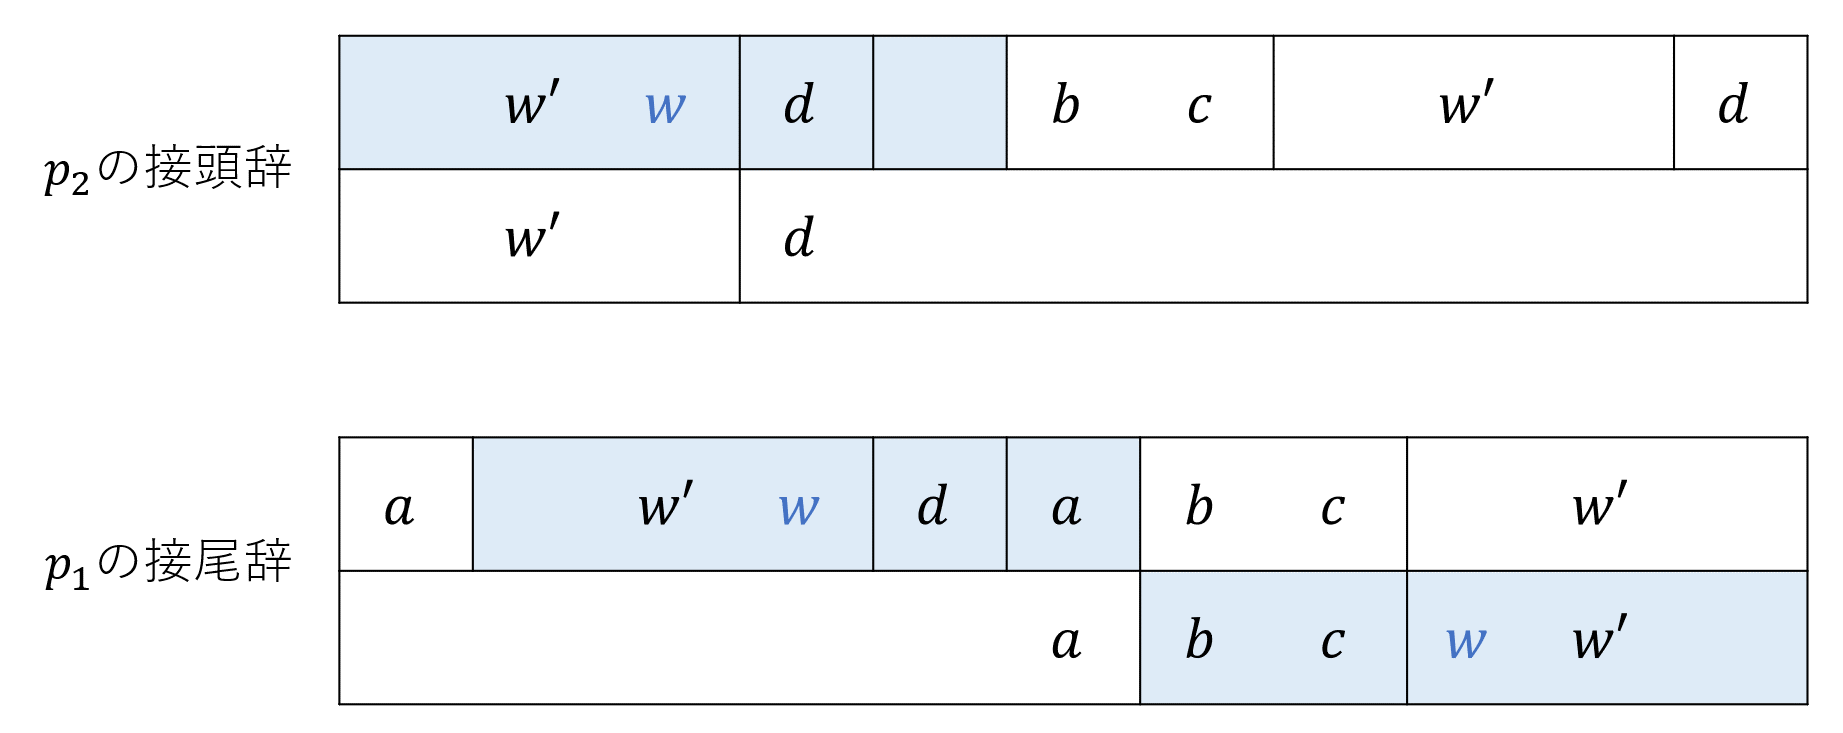
\includegraphics[width=\linewidth]{画像/追加部分1.png}
\caption{\scriptsize $|w| = |w^{\prime}|+2$における$p_{1}$の接尾辞,$p_{2}$の接頭辞の関係}
\label{追加部分1}
\end{figure}

図\ref{追加部分1}のように,$w=w^{\prime}da,w=bcw^{\prime}$となる.
よって,$w^{\prime}da=bcw^{\prime}$となる.

\begin{cl}\label{主張1}
$w^{\prime}$を定数記号列,a,b,c,dを定数記号とする.
このとき,$w^{\prime}da \not =bcw^{\prime} (b \not = a,d,c \not = a,d)$となる.
\end{cl}
\begin{proof}
$w^{\prime}da=bcw^{\prime}$と仮定すると,$w^{\prime}=bcw_{1}da (w_{1}は定数記号列)$とおける.
$w^{\prime}da=bcw_{1}dada, bcw^{\prime}=bcbcw_{1}da$であるので,$bcw_{1}dada=bcbcw_{1}da$となる.
$w^{\prime}$と同様に$w_{1}$を考えると,$w_{1}=bcw_{2}da (w_{2}は定数記号列)$とおける.
$w_{2}$以降も同様に定義できる.
ここで,定数記号列の長さを考えていくと,$|w_{1}|=|w^{\prime}|-4, |w_{2}|=|w_{1}|-4$のように,$|w_{i+1}|$は$|w_{i}|$より長さ4ずつ短くなっていく.
そのため,定数記号列を繰り返し定義していくと,最終的に定義できる$w_{n}$は長さ0,1,2,3のいずれかとなる.

\begin{figure}[H]
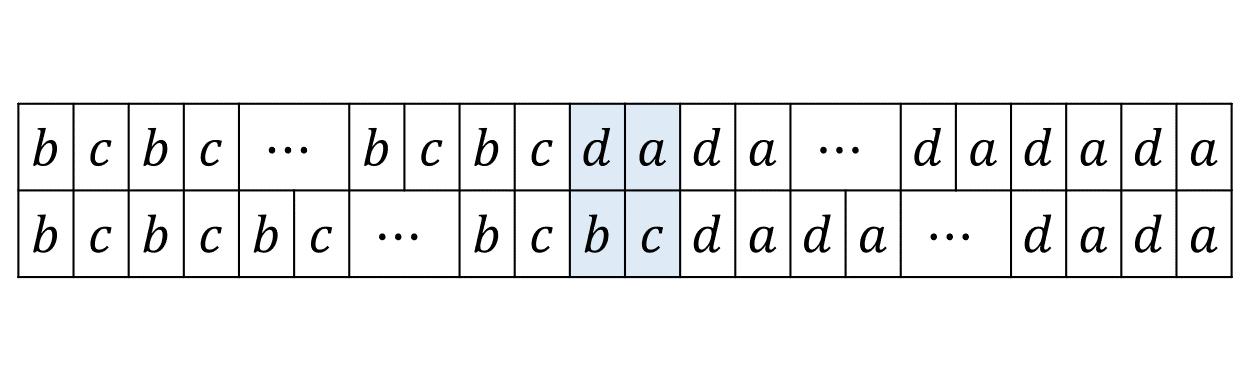
\includegraphics[width=\linewidth]{画像/追加部分2.png}
\caption{$|w_{n}| = 0$における定数記号列}
\label{追加部分2}
\end{figure}

$|w_{n}|=0$のとき,図\ref{追加部分2}のように,$da=bc$となる.
これは,$b \not = d$であることに矛盾する.

\begin{figure}[H]
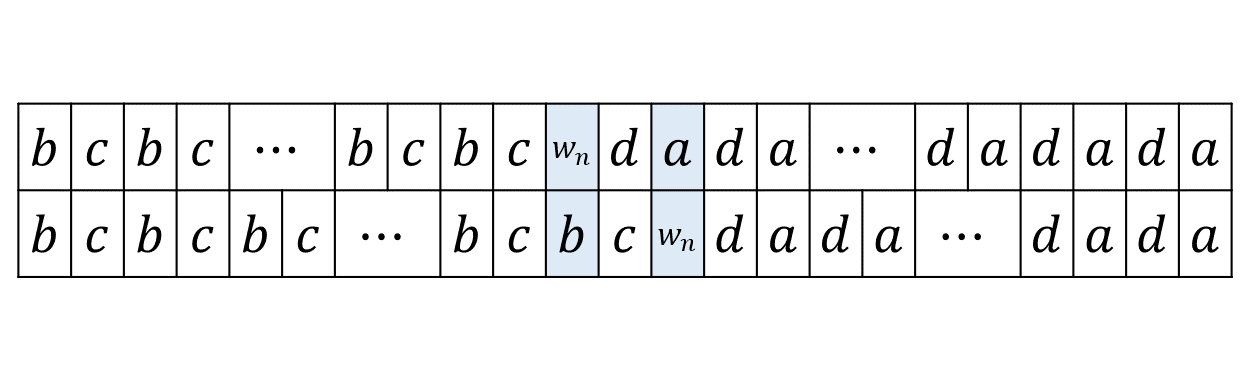
\includegraphics[width=\linewidth]{画像/追加部分3.png}
\caption{$|w_{n}| = 1$における定数記号列}
\label{追加部分3}
\end{figure}

$|w_{n}|=1$のとき,図\ref{追加部分3}のように,$w_{n}=a=b$となる.
これは,$b \not = a$であることに矛盾する.

\begin{figure}[H]
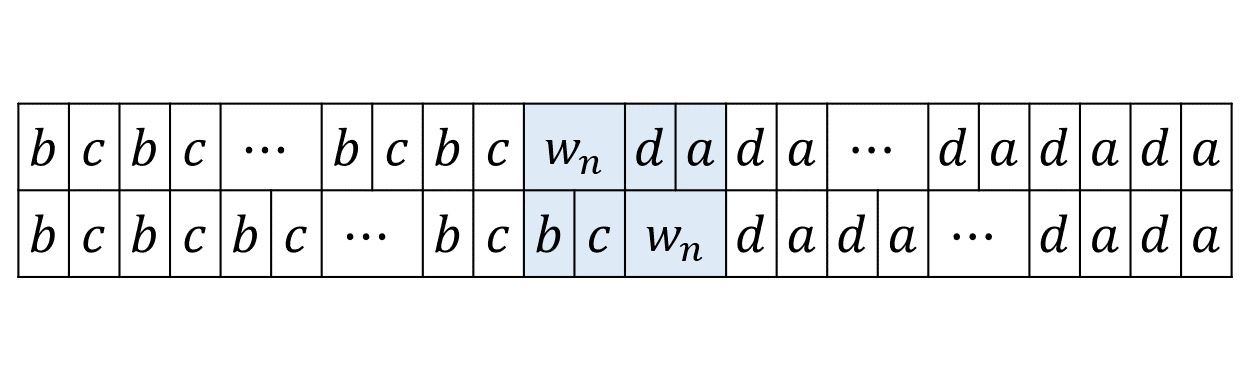
\includegraphics[width=\linewidth]{画像/追加部分4.png}
\caption{$|w_{n}| = 2$における定数記号列}
\label{追加部分4}
\end{figure}

$|w_{n}|=2$のとき,図\ref{追加部分4}のように,$w_{n}=bc=da$となる.
これは,$b \not = d$であることに矛盾する.

\begin{figure}[H]
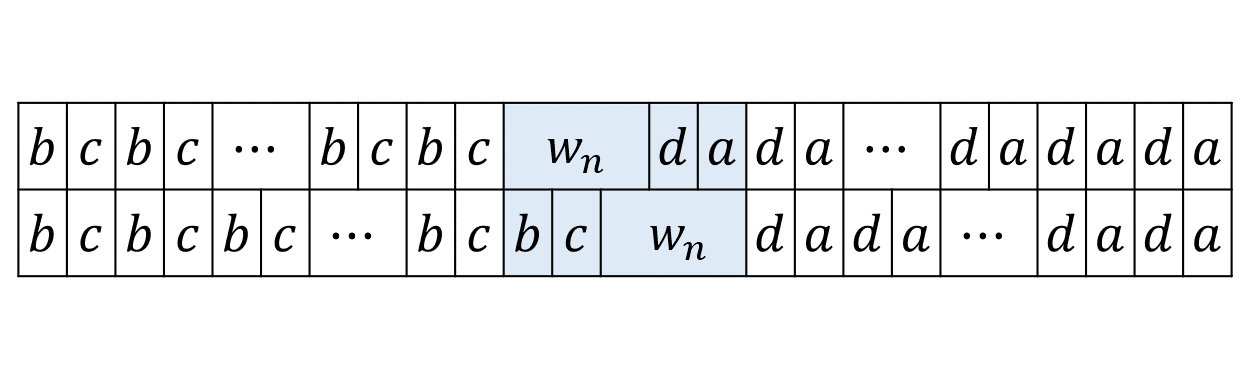
\includegraphics[width=\linewidth]{画像/追加部分5.png}
\caption{$|w_{n}| = 3$における定数記号列}
\label{追加部分5}
\end{figure}

$|w_{n}|=3$のとき,$w_{n}=w_{n_{1}}w_{n_{2}}w_{n_{3}} (w_{n_{i}}はw_{n}におけるi番目の定数記号)$と表すと,図\ref{追加部分5}のように,$bcw_{n_{3}}=w_{n_{1}}da$となる.
よって,$c=d$となる.
これは,$c \not = d$であることに矛盾する.

以上より,$|w_{n}|=0,1,2,3$のとき,すべてにおいて矛盾するため,$w^{\prime}da \not = bcw^{\prime}$となる.
\end{proof}
主張\ref{主張1}より,$w^{\prime}da=bcw^{\prime}$は$w^{\prime}da \not =bcw^{\prime}$であることに矛盾する.

\begin{figure}[H]
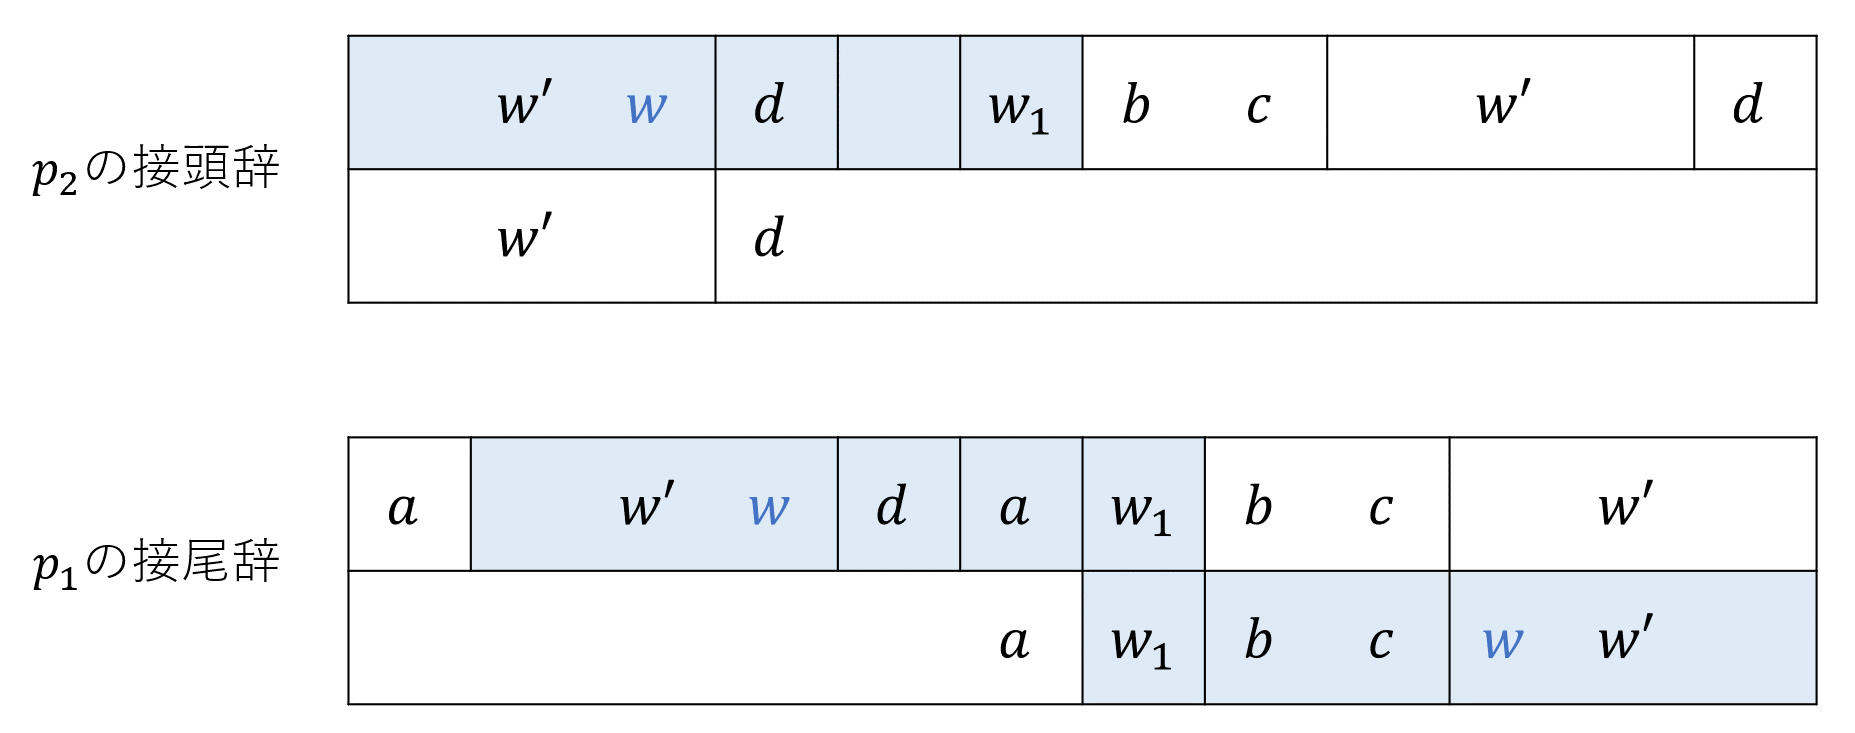
\includegraphics[width=\linewidth]{画像/追加部分6.png}
\caption{\scriptsize $|w| \ge |w^{\prime}|+3$における$p_{1}$の接尾辞,$p_{2}$の接頭辞の関係}
\label{追加部分6}
\end{figure}

$|w| \ge |w^{\prime}|+3$であれば,図\ref{追加部分6}のように,$w=w^{\prime}daw_{1}=w_{1}bcw^{\prime} (w_{1}は定数記号列)$となる.
よって,$w^{\prime}daw_{1}=w_{1}bcw^{\prime}$となる.

\begin{cl}\label{主張2}
$w, w_{1}$を定数記号列,a,b,c,dを定数記号とする.
このとき,$wdaw_{1} \not =w_{1}bcw (b \not = a,d,c \not = a,d)$となる.
\end{cl}
\begin{proof}
$wdaw_{1}=w_{1}bcw$と仮定する.

$|w_{1}| \le |w| \le |w_{1}|+2$であるときを考えると,

\begin{figure}[H]
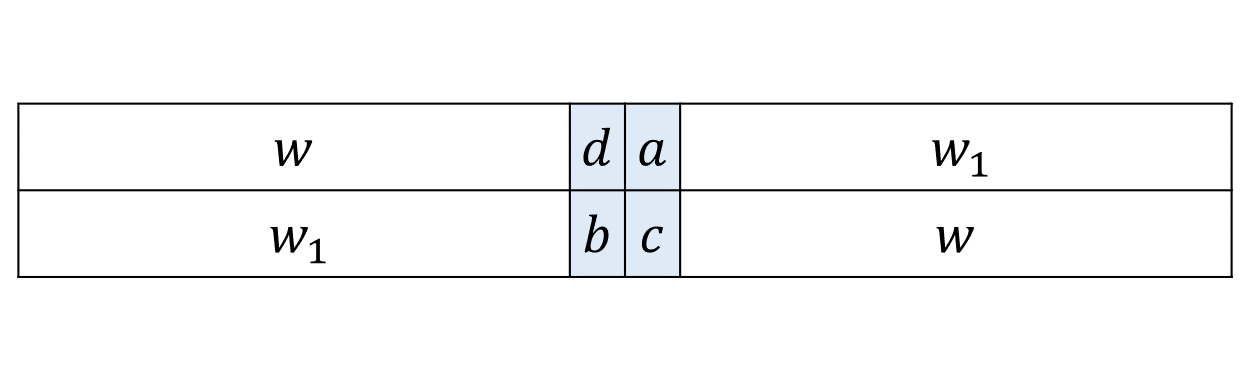
\includegraphics[width=\linewidth]{画像/追加部分7.png}
\caption{$|w| = |w_{1}|$における定数記号列}
\label{追加部分7}
\end{figure}

$|w|=|w_{1}|$であれば,図\ref{追加部分7}のように,$bc=da$となる.
これは,$b \not = d$であることに矛盾する.

\begin{figure}[H]
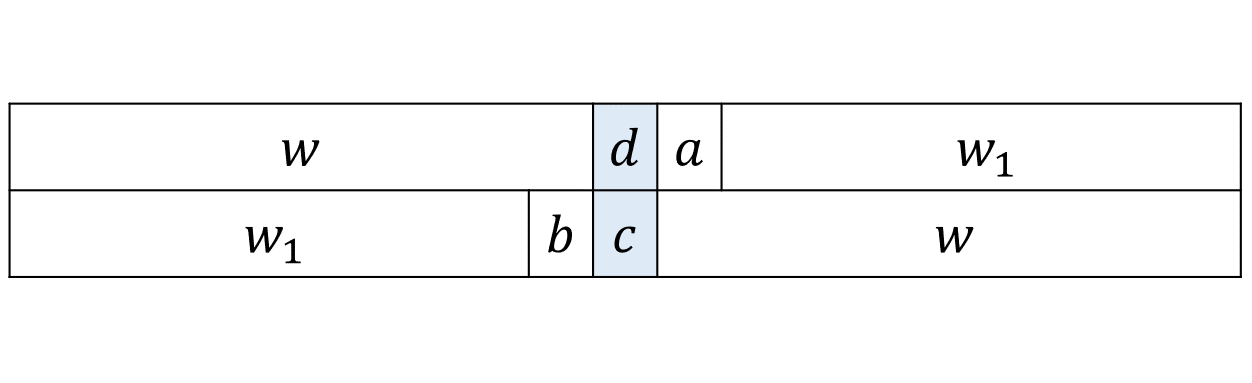
\includegraphics[width=\linewidth]{画像/追加部分8.png}
\caption{$|w| = |w_{1}|+1$における定数記号列}
\label{追加部分8}
\end{figure}

$|w|=|w_{1}|+1$であれば,図\ref{追加部分8}のように,$c=d$となる.
これは,$c \not = d$であることに矛盾する.

\begin{figure}[H]
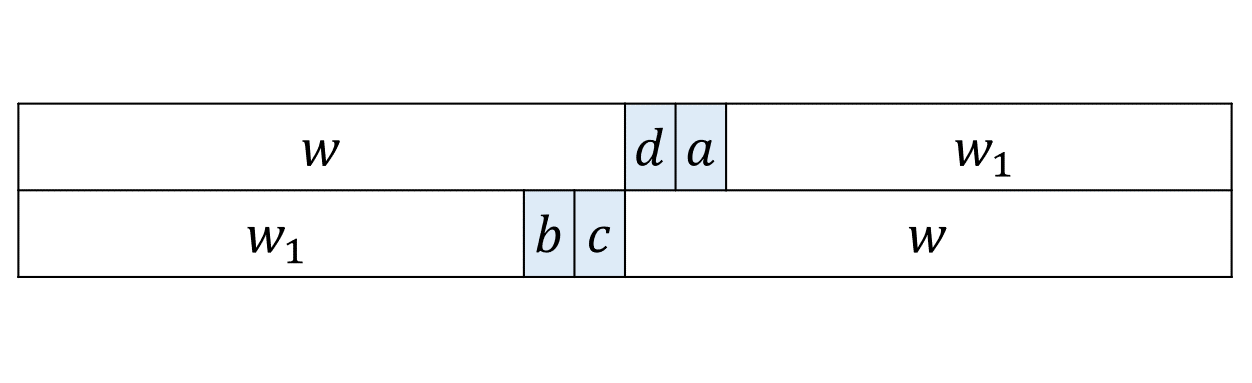
\includegraphics[width=\linewidth]{画像/追加部分9.png}
\caption{$|w| = |w_{1}|+2$における定数記号列}
\label{追加部分9}
\end{figure}

$|w|=|w_{1}|+2$であれば,図\ref{追加部分9}のように,$w=w_{1}bc=daw_{1}$となる.
これは,主張\ref{主張1}より,矛盾する.

次に,$2|w_{1}| \le |w| \le 2|w_{1}|+4$であるときを考えると,

\begin{figure}[H]
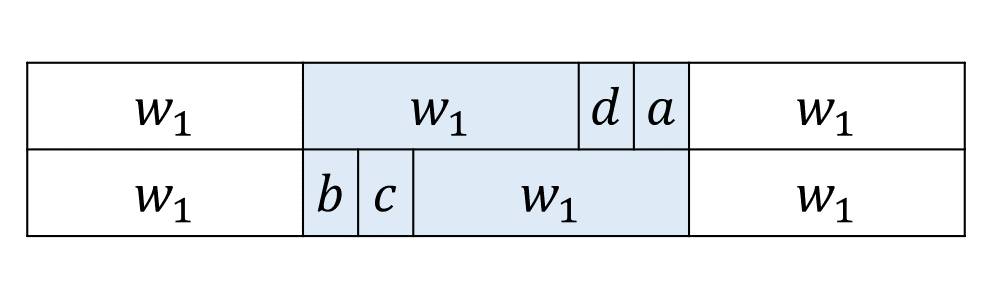
\includegraphics[width=\linewidth]{画像/追加部分14.png}
\caption{$|w| = 2|w_{1}|$における定数記号列}
\label{追加部分14}
\end{figure}

$|w|=2|w_{1}|$であれば,図\ref{追加部分14}のように,$w_{1}da=bcw_{1}$となる.
これは,主張\ref{主張1}より,矛盾する.

\begin{figure}[H]
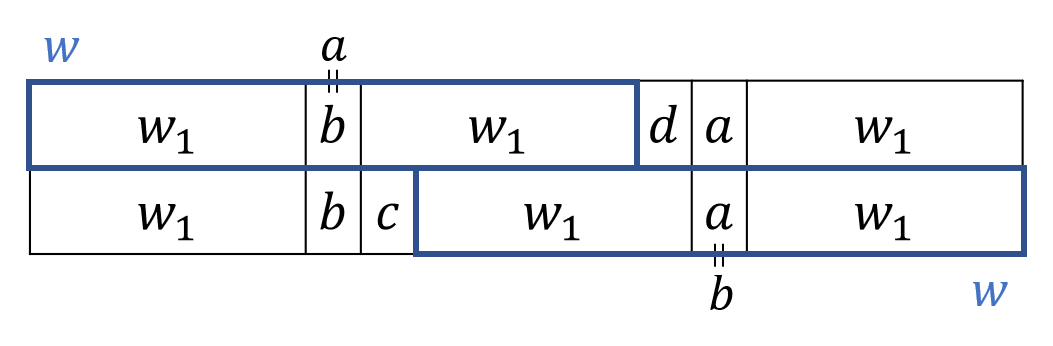
\includegraphics[width=\linewidth]{画像/追加部分13.png}
\caption{$|w| = 2|w_{1}|+1$における定数記号列}
\label{追加部分13}
\end{figure}

$|w|=2|w_{1}|+1$であれば,図\ref{追加部分13}のように,$b=a$となる.
これは,$b \not = a$であることに矛盾する.

\begin{figure}[H]
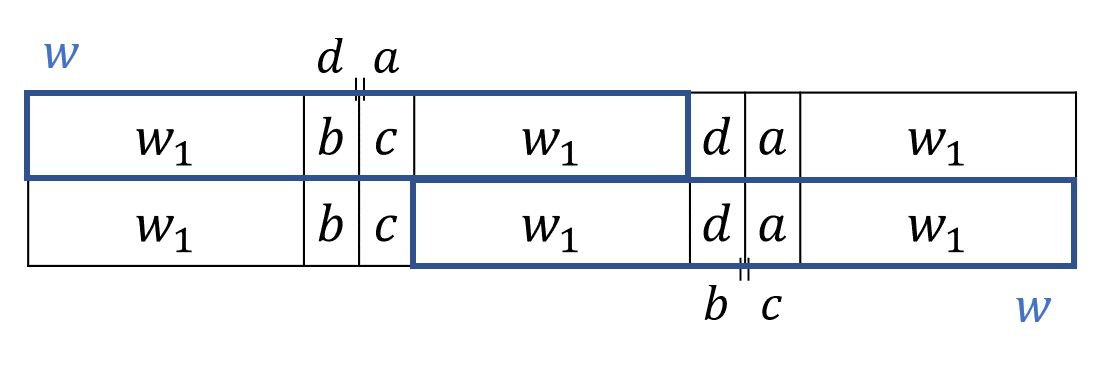
\includegraphics[width=\linewidth]{画像/追加部分12.png}
\caption{$|w| = 2|w_{1}|+2$における定数記号列}
\label{追加部分12}
\end{figure}

$|w|=2|w_{1}|+2$であれば,図\ref{追加部分12}のように,$bc=da$となる.
これは,$b \not = d$であることに矛盾する.

\begin{figure}[H]
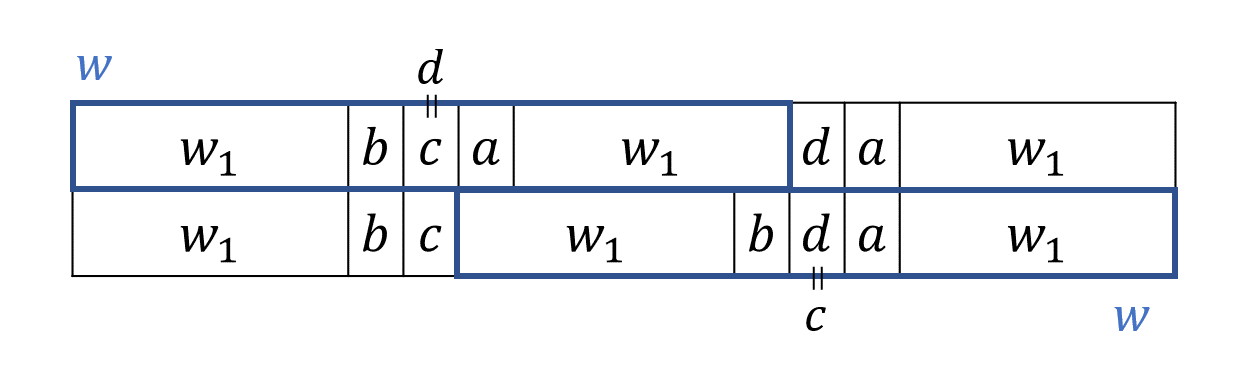
\includegraphics[width=\linewidth]{画像/追加部分11.png}
\caption{$|w| = 2|w_{1}|+3$における定数記号列}
\label{追加部分11}
\end{figure}

$|w|=2|w_{1}|+3$であれば,図\ref{追加部分11}のように,$c=d$となる.
これは,$c \not = d$であることに矛盾する.

\begin{figure}[H]
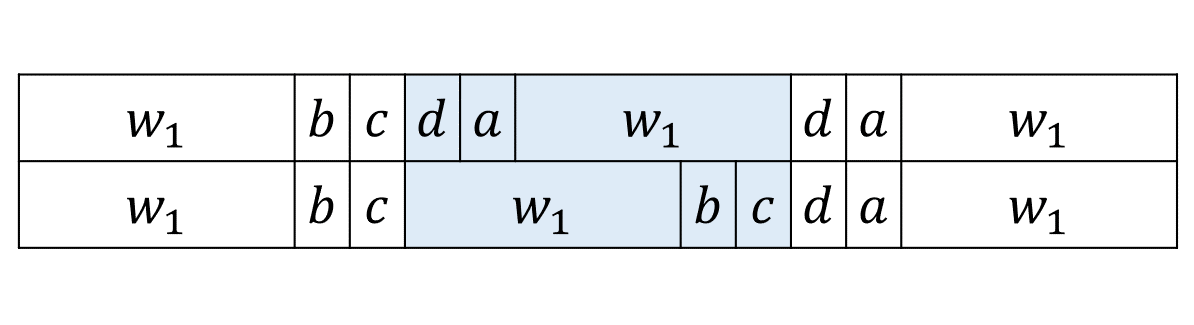
\includegraphics[width=\linewidth]{画像/追加部分10.png}
\caption{$|w| = 2|w_{1}|+4$における定数記号列}
\label{追加部分10}
\end{figure}

$|w|=2|w_{1}|+4$であれば,$w=w_{1}bcdaw_{1}$とおける.
図\ref{追加部分10}のように,$daw_{1}=w_{1}bc$となる.
これは,主張\ref{主張1}より,矛盾する.

上記以外の$|w_{1}|+3 \le |w| \le 2|w_{1}|-1, |w| \ge 2|w_{1}|+5$の場合,対象とする$w,w_{1}$の長さを減らして考えることができる.

$|w_{1}|+3 \le |w| \le 2|w_{1}|-1$のとき,

\begin{figure}[H]
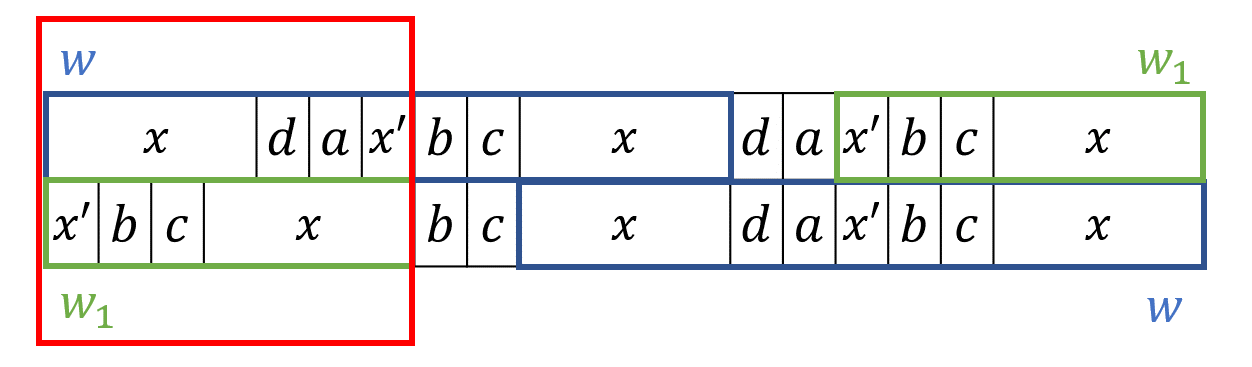
\includegraphics[width=\linewidth]{画像/w1+3.png}
\caption{\scriptsize $|w_{1}|+3 \le |w| \le 2|w_{1}|-1$における定数記号列}
\label{w1+3}
\end{figure}

図\ref{w1+3}のように,$x$を$w$,$x^{\prime}$を$w_{1}$と置き換えて考えることができる.
よって,赤枠部分以外の定数文字列を無視できるため,対象とする定数文字列の長さを減らすことができる.

$|w| \ge 2|w_{1}|+5$のとき,

\begin{figure}[H]
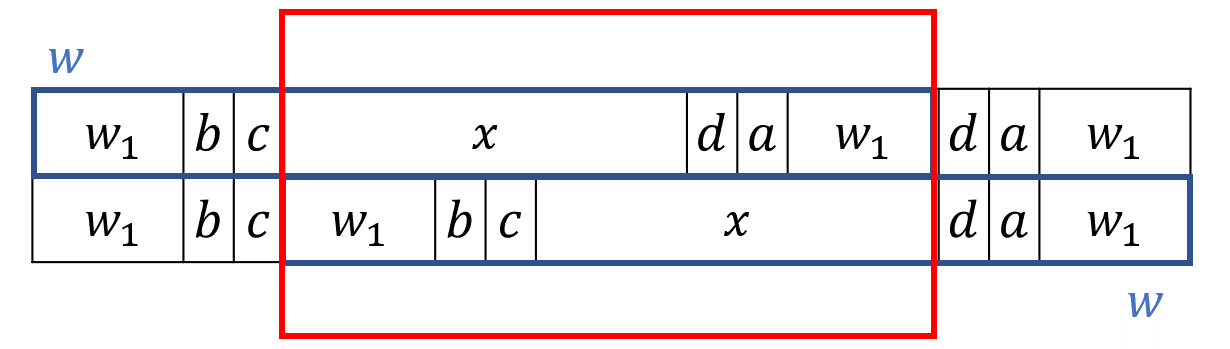
\includegraphics[width=\linewidth]{画像/2w1+5.png}
\caption{\scriptsize $|w| \ge 2|w_{1}|+5$における定数記号列}
\label{2w1+5}
\end{figure}

図\ref{2w1+5}より,$x$と$w$を置き換えて考えることができる.
よって,赤枠部分以外の定数文字列を無視できるため,対象とする定数文字列の長さを減らすことができる.

したがって,$|w_{1}|+3 \le |w| \le 2|w_{1}|-1, |w| \ge 2|w_{1}|+5$の場合,$w,w_{1}$の長さを減らして考えることができる.
最終的に,$|w_{1}| \le |w| \le |w_{1}|+2,2|w_{1}| \le |w| \le 2|w_{1}|+4,|w_{1}|=0$のいずれかに当てはまる.
\end{proof}
主張\ref{主張2}より,$w^{\prime}daw_{1}=w_{1}bcw^{\prime}$は$w^{\prime}daw_{1}\not =w_{1}bcw^{\prime}$であることに矛盾する.

$|w| \le |w^{\prime}|$である場合も同様に証明できる.
\end{proof}
補題\ref{追加部分}の証明より,次の系が成り立つ.

\begin{col}
$\sharp \Sigma \ge 3$とし,$p, q$を正規パターンとする.
正規パターンの有限集合$D= \{ ya, bc, dy \} (b = a または,c = d)$で表されるとき,すべての$r \in D$に対して$p \{ x := r \} \preceq q$ならば,$p \{ x := xy \} \not \preceq q$である正規パターン$q$が存在する.
\end{col}

\begin{ex}
$p=eabcbcadabcbcadaxbcadabcbcadade$

$q=y_{1}abcbcadabcbcadady_{2}$

\begin{eqnarray*}
&p& \{ x:=ya \} \\ 
& = & (eabcbcadabcbcaday)abcbcadabcbcadade\\
& = & q \{ y_{1} := eabcbcadabcbcaday_{1} \} \\
& \preceq & q,\\
&p& \{ x:=bc \}  \\
& = & (eabcbcad)abcbcadabcbcadad(abcbcadade) \\
& = & q \{ y_{1} := eabcbcad,y_{2} := abcbcadade \} \\
& \preceq & q,\\
&p& \{ x:=dy \}  \\
& = & eabcbcadabcbcadad(ybcadadabcbcadade) \\
& = & q \{ y_{2} := y_{2}bcadadabcbcadade \} \\
& \preceq & q.
\end{eqnarray*}

\end{ex}

\begin{lem}[Sato et al.\cite{Sato1}]\label{補題15}
$\sharp \Sigma \ge 3$とし,$p,q$を正規パターンとする.
このとき,ある$a \in \Sigma$に対して,
$p \{ x := a \} \preceq q$かつ$p \{ x := xy \} \preceq q$ならば$p \preceq q$である.
ただし,$y$は$q$に含まれない変数記号である.
\end{lem}

%\begin{lem}\label{追加補題1}
%$k \ge 3$,$m \ge \sqrt{k+1}$,$\sharp \Sigma \ge k+m$,$P \in \RPatplus$,$Q \in \RPat^{k}$とする.
%すべての定数記号$a, b \in \Sigma$に対し,ある正規パターン$q \in Q$が存在し,
%$p \{ x:=ab \} \preceq q$ならば,$p \{ x:=xy \} \preceq q$となる.
%\end{lem}

\begin{lem}\label{追加補題1}
$k \ge 4$,$\sharp \Sigma \ge k+3$,$P \in \RPatplus$,$Q \in \RPat^{k}$とする.
すべての定数記号$a, b \in \Sigma$に対し,ある正規パターン$q \in Q$が存在し,
$p \{ x:=ab \} \preceq q$ならば,$p \{ x:=xy \} \preceq q$となる.
\end{lem}
\begin{proof}
$p$に変数記号が現れない場合は自明である.
したがって,$p=p_{1}xp_{2}$ ($p_{1},p_{2}$は正規パターン,$x$は変数記号)とおく.
また,$Q=\{ q_{1}, \ldots , q_{k} \}$とする.次のように記号を定める.
\begin{align*}
A_{i} & = \{ a \in \Sigma \mid p \{ x:=ay \} \preceq q_{i},\ y\in X\},\\ 
B_{i} & = \{ b \in \Sigma \mid p \{ x:=yb \} \preceq q_{i},\ y\in X\},\\ 
A & = \bigcup_{i=1}^{k}A_{i},\\
B & = \bigcup_{i=1}^{k}B_{i},\\
\tilde{A} & = \Sigma\setminus A,\\
\tilde{B} & = \{ \bar{b} \mid b \in \Sigma \setminus B \},\\
\bar{\Sigma} & = \{ \bar{c} \mid c \in \Sigma \}~~(i=1, \ldots , k).
\end{align*}
$p \{ x:=xy \} \not \preceq q_{i}$ \ ($i=1, \ldots , k$)と仮定する.
ある$i$に対して,$\sharp A_{i} \ge 2$または$\sharp B_{i} \ge 2$のとき,補題\ref{補題14} (i)により,$p \{ x:=xy \} \preceq q_{i}$となる.
これは仮定に矛盾する.よって,全ての$i$ ($i=1, \ldots , k$)に対して,$\sharp A_{i} \le 1$かつ$\sharp B_{i} \le 1$となる.
したがって,$0 \le \sharp A \le k$かつ$0 \le \sharp B \le k$となり,$3 \le \sharp \tilde{A} \le k+3$かつ$3 \le \sharp \tilde{B} \le k+3$となる.

$G=(\Sigma,\bar{\Sigma}; \tilde{A} \times \tilde{B})$
を$\Sigma$と$\bar{\Sigma}$を部集合とし,辺集合を$\tilde{A} \times \tilde{B}$とする2部グラフとする.
$\Sigma$と$\bar{\Sigma}$を部集合とし,$\tilde{E}_{i}=\{ (a, \bar{b}) \in \tilde{A} \times \tilde{B} \mid p \{ x:=ab \} \preceq q_{i} \}$を辺集合とする2分グラフを$\tilde{G}_{i}=(\Sigma,\bar{\Sigma}; \tilde{E}_{i})$とする.

\begin{figure}[H]
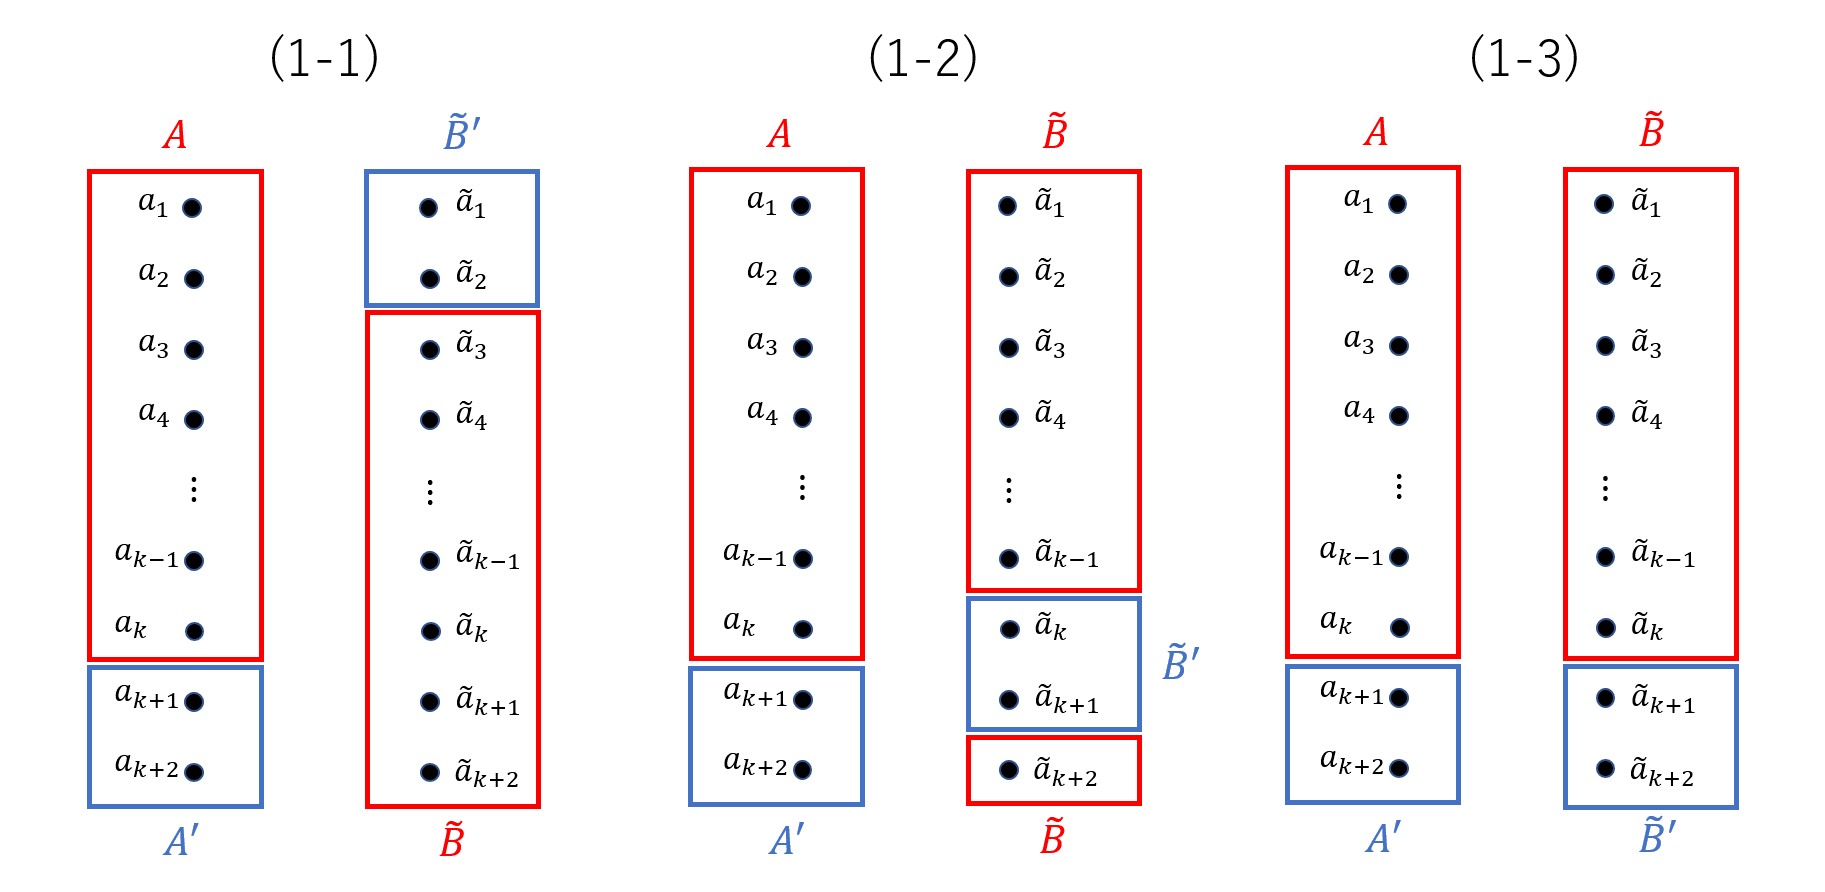
\includegraphics[width=\linewidth]{画像/グラフ比較.png}
\caption{\scriptsize $A,B,\tilde{A},\tilde{B}$に含まれる要素によるグラフの違い}
\label{グラフ比較}
\end{figure}

まず,$\sharp A=\sharp B$である場合から考える.
$\sharp A=k,\sharp B=k$のとき,図\ref{グラフ比較}パターン1の場合,$G$に含まれる辺は,$\sharp\tilde{A} \times \sharp\tilde{B}=3 \times 3=9$本となる.
図\ref{グラフ比較}パターン2の場合,$G$に含まれる辺の最大$\tilde{A}+\tilde{B}=6$本が系のようなパターンとなる.
よって,$G$に含まれる辺の$9-6=3$本は,補題\ref{追加補題1}のようにパターンとなる.
したがって,ある$i$に対して,$p \{ x:=xy \} \preceq q_{i}$となる.
これは,仮定に矛盾する.

$\sharp A=k-1,\sharp B=k-1$のとき,$G$に含まれる辺は,$\sharp\tilde{A} \times \sharp\tilde{B}=4 \times 4=16$本となる.
図\ref{グラフ比較}パターン2のような場合,$\sharp A_{i}=1,\sharp B_{i}=1 (i=1, \ldot , k-1)$である$\tilde{G}_{i}$に含まれる辺は最大8本となる.
よって,$\tilde{G}_{k}$には$16-8=8$本の辺が含まれる.
$\tilde{G}_{k}$に次数が3以上である頂点$a$が存在するとき,補題\ref{補題10}より,$p \{x:=ay \} \preceq q_{k}$または$p \{ x:= ya \} \preceq q_{k}$となり,$A_{k}$または$B_{k}$の定義に矛盾する.
したがって,$\tilde{G}_{k}$に含まれる頂点の次数は2以下となる.

\begin{figure}[H]
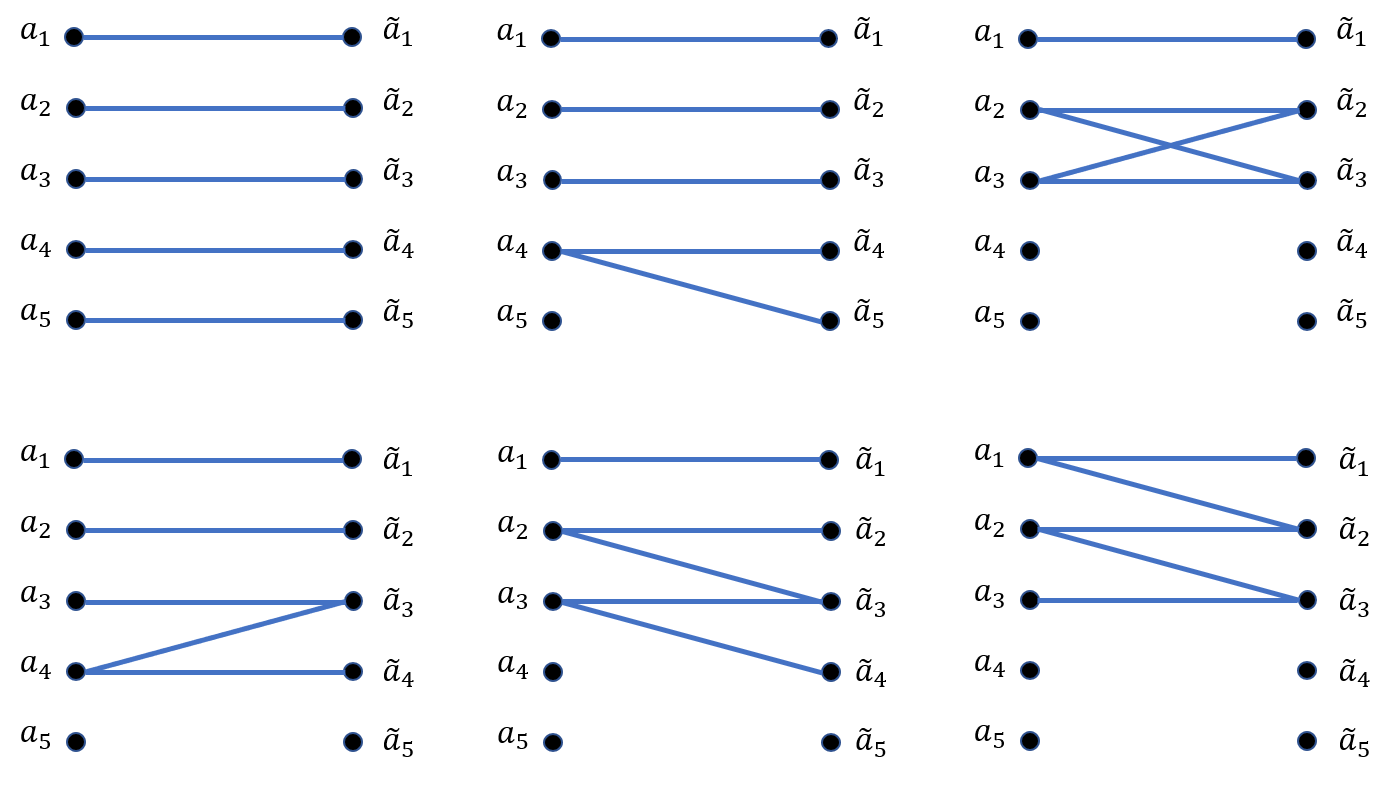
\includegraphics[width=\linewidth]{画像/辺5本の場合.png}
\caption{\scriptsize 辺数が5である二分グラフの例(各頂点の次数は2以下)}
\label{辺5本の場合}
\end{figure}

図\ref{辺5本の場合}のように,ある$i$に対して,$\tilde{G}_{i}$に含まれる辺が5本以上であるとき,互いに隣接しない辺が3本以上存在する.
よって,補題\ref{補題14}より,$p \{x:=xy \} \preceq q_{i}$となる.
これは,仮定に矛盾する.

$\sharp A=k-2,\sharp B=k-2$のとき,$G$に含まれる辺は,$\sharp\tilde{A} \times \sharp\tilde{B}=5 \times 5=25$本となる.
$\sharp A_{i}=1,\sharp B_{i}=1 (i=1, \ldots , k-2)$である$\tilde{G}_{i}$に含まれる辺は最大10本となる.
よって,$\tilde{G}_{k-1},\tilde{G}_{k}$には合計で辺が$25-10=15$本含まれる.
したがって,$15 \ge 4 \times 2 + 1$であるため,$\tilde{G}_{k-1}$または$\tilde{G}_{k}$に含まれる辺は5本以上となり,互いに隣接しない辺が3本以上存在する.
よって,補題\ref{補題14}より,$p \{x:=xy \} \preceq q_{i}$となる.
これは,仮定に矛盾する.

$0 \le \sharp A \le k-3,0 \le \sharp B \le k-3$のとき,$G$の辺の総数は$\sharp\tilde{A} \times \sharp\tilde{B}$となる.
そのうち,図\ref{グラフ比較}パターン2のような場合,$\sharp A_{i}=1,\sharp B_{i}=1$までの$\tilde{G}_{i}$に最大で$\sharp\tilde{A}+\sharp\tilde{B}$本含まれる.
このとき,$\sharp A_{j}=0,\sharp B_{j}=0$である$\tilde{G}_{j}$に$\sharp\tilde{A} \times \sharp\tilde{B} - (\sharp\tilde{A} + \sharp\tilde{B})$本の辺が含まれる.
\begin{align*}
&\sharp\tilde{A} \times \sharp\tilde{B} -(\sharp\tilde{A}+\sharp{B}) \ge 4(\sharp\tilde{A}-3)+1\\
&\sharp\tilde{A}^{2}-2\sharp\tilde{A} \ge 4\sharp\tilde{A}-12+1\\
&\sharp\tilde{A}^{2}-2\sharp\tilde{A}-4\sharp\tilde{A}+11 \ge 0\\
&\sharp\tilde{A}^{2}-6\sharp\tilde{A}+11 \ge 0
\end{align*}
二次不等式の判別式をDとすると,$D=36-4\times11=-8$となる.
$D<0$より,すべての$\sharp\tilde{A}$について不等式が成り立つ.
よって,$0 \le \sharp A \le k-3,0 \le \sharp B \le k-3$においても,ある$i$に対して,$\sharp A_{i}=0,\sharp B_{i}=0$である$\tilde{G}_{i}$に含まれる辺は5本以上となり,互いに隣接しない辺が3本以上存在する.
したがって,補題\ref{補題14}より,$p \{x:=xy \} \preceq q_{i}$となる.
これは,仮定に矛盾する.

次に,$\sharp A \not = \sharp B$である場合を考える.
$\sharp A \not = \sharp B$であれば,$\sharp A_{i}=1,\sharp B_{i}=0$または,$\sharp A_{i} =0,\sharp B_{i}=1$となる$i$が存在する.

\begin{figure}[H]
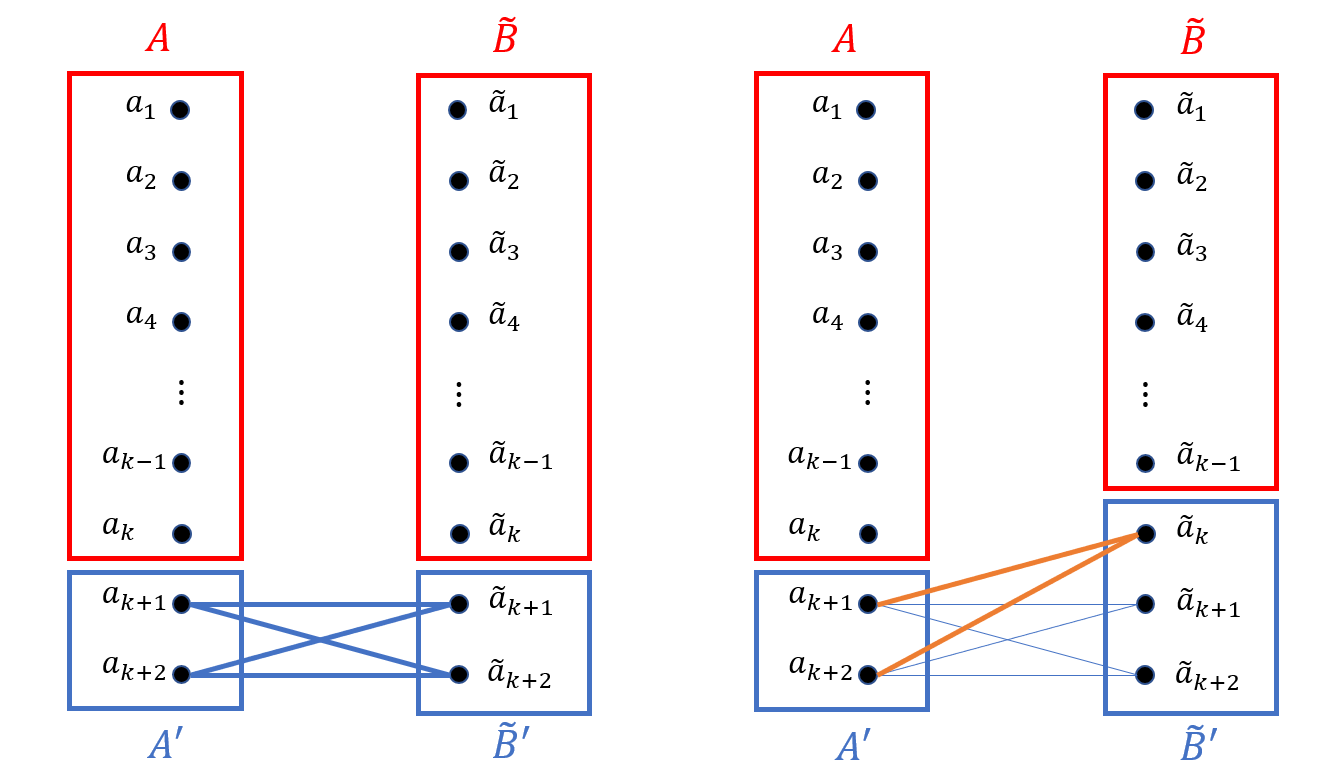
\includegraphics[width=\linewidth]{画像/abが異なる場合.png}
\caption{\scriptsize $\sharp A_{k} =1,\sharp B_{k}=1$の場合と$\sharp A_{k}=1,\sharp B_{k}=0$の場合の辺数の違い}
\label{abが異なる場合}
\end{figure}

$\sharp A_{i}=1,\sharp B_{i}=0$の場合は,図\ref{abが異なる場合}のように,$\sharp A_{i} =1,\sharp B_{i}=1$の場合と比べて,$G$に含まれる辺数は$\sharp\tilde{A}$本多くなる.

\begin{figure}[H]
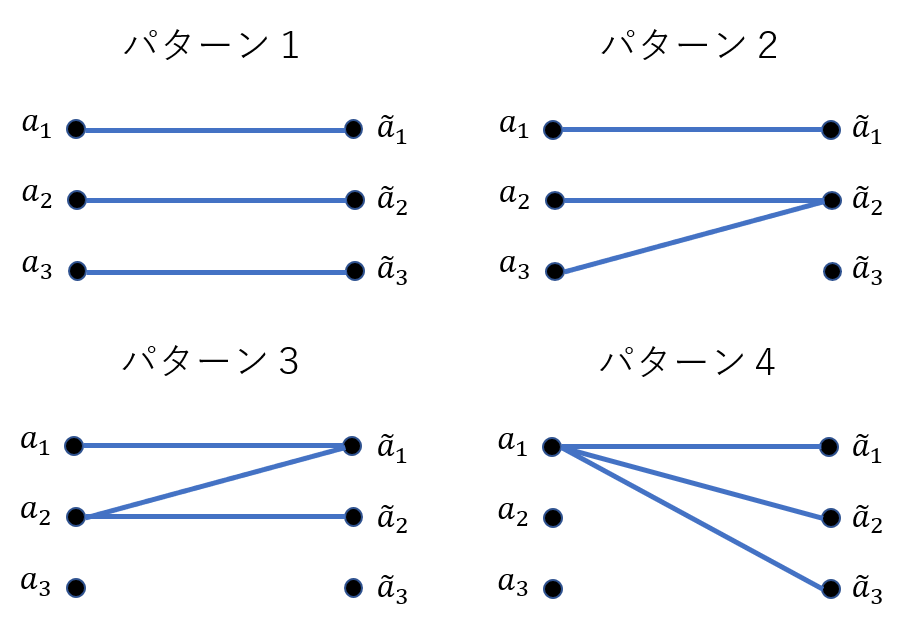
\includegraphics[width=\linewidth]{画像/辺3におけるパターン.png}
\caption{\scriptsize 辺数が3である二分グラフの例(各頂点の次数は2以下)}
\label{辺3におけるパターン}
\end{figure}

$\tilde{G}_{i}$に含まれる辺数が3であるとき,図\ref{辺3におけるパターン}のように2つのパターンが存在する.
パターン1の場合,補題\ref{補題14}(abc)より,$p \{ x:=xy \} \preceq q_{i}$となる.
パターン2の場合,互いに隣接しない辺が2本存在する.
補題\ref{補題14}(d)より,$p \{ x:=xy \} \preceq q_{i}$となり,$\sharp A_{i}=1,\sharp B_{i}=0$であれば,$\tilde{G}_{i}$に含まれる辺数が2以下となる.
よって,$\sharp\tilde{A} \ge 2$より,$G$に含まれる辺数が減ることはない.
$\sharp A_{i}=0,\sharp B_{i}=1$の場合も同様に考えられるため,$\sharp A \not = \sharp B$においても,仮定に矛盾する.
\end{proof}

\begin{comment}
$\sharp A=k-2,\sharp B=k-2$のとき,$\sharp A_{i}=0,\sharp B_{i}=0 (i=k-1,k)$である$\tilde{G}_{i}$にはそれぞれ平均で$15÷2=7.5$本の辺が含まれる.
$\sharp A,\sharp B$の数が1ずつ減ったとき,$G$に含まれる辺は,$\sharp \tilde{A} +\sharp \tilde{B} -1$本増える.
\begin{align*}
&\sharp \tilde{A} + \sharp \tilde{B} -3 \ge \tfrac{(\sharp\tilde{A}-1)(\sharp\tilde{B}-1)-(\sharp\tilde{A}-1+\sharp\tilde{B}-1)}{(\sharp\tilde{A}-1)-3} \\
&2\sharp\tilde{A}-3 \ge \tfrac{(\sharp\tilde{A}-1)(\sharp\tilde{A}-1)-(2\sharp\tilde{A}-2)}{\sharp\tilde{A}-4}\\
&2\sharp\tilde{A}-3 \ge \tfrac{\sharp\tilde{A}^{2}-2\sharp\tilde{A}+1-2\sharp\tilde{A}+2}{\sharp\tilde{A}-4}\\
&(2\sharp\tilde{A}-3)(\sharp\tilde{A}-4) \ge \sharp\tilde{A}^{2}-4\sharp\tilde{A}+3\\
&2\sharp\tilde{A}^{2}-11\sharp\tilde{A}+12 \ge \sharp\tilde{A}^{2}-4\sharp\tilde{A}+3\\
&\sharp\tilde{A}^{2}-7\sharp\tilde{A}+9 \ge 0\\
&\sharp\tilde{A} \le \tfrac{7-\sqrt{13}}{2},\tfrac{7+\sqrt{13}}{2} \le \sharp\tilde{A}
\end{align*}

$\sharp\tilde{A} \ge 3$より,$\tfrac{7+\sqrt{13}}{2} \le \sharp\tilde{A}$となる.
$\tfrac{7+3}{2} \le \tfrac{7+\sqrt{13}}{2} \le \tfrac{7+4}{2}$より,$5 \le \tfrac{7+\sqrt{13}}{2} \le 5.5$であり,$6 \le \sharp\tilde{A}$となる.
$\sharp A \ge k-3, \sharp B \ge k-3$のとき,$\sharp\tilde{A}=k+3-\sharp{A}=k+3-(k-3)=6$以上となる.
よって,$\sharp A \ge k-3, \sharp B \ge k-3$のとき,$\sharp A_{i}=0,\sharp B_{i}=0$である$\tilde{G}_{i}$にはそれぞれ平均で$7.5$本以上の辺が含まれることになる.
したがって,ある$i$に対して,$\tilde{G}_{i}$に含まれる辺は5本以上となり,互いに隣接しない辺が3本以上存在する.
補題\ref{補題14}より,$p \{x:=xy \} \preceq q_{i}$となる.
これは,仮定に矛盾する.
\end{comment}

\begin{lem}\label{kが3以下}
$k \le 3$,$\sharp \Sigma \ge k+2$,$P \in \RPatplus$,$Q \in \RPat^{k}$とする.
すべての定数記号$a, b \in \Sigma$に対し,ある正規パターン$q \in Q$が存在し,
$p \{ x:=ab \} \preceq q$ならば,$p \{ x:=xy \} \preceq q$となる.
\end{lem}
\begin{proof}
$p$に変数記号が現れない場合は自明である.
したがって,$p=p_{1}xp_{2}$ ($p_{1},p_{2}$は正規パターン,$x$は変数記号)とおく.
また,$Q=\{ q_{1}, \ldots , q_{k} \}$とする.次のように記号を定める.
\begin{align*}
A_{i} & = \{ a \in \Sigma \mid p \{ x:=ay \} \preceq q_{i},\ y\in X\},\\ 
B_{i} & = \{ b \in \Sigma \mid p \{ x:=yb \} \preceq q_{i},\ y\in X\},\\ 
A & = \bigcup_{i=1}^{k}A_{i},\\
B & = \bigcup_{i=1}^{k}B_{i},\\
\tilde{A} & = \Sigma\setminus A,\\
\tilde{B} & = \{ \bar{b} \mid b \in \Sigma \setminus B \},\\
\bar{\Sigma} & = \{ \bar{c} \mid c \in \Sigma \}~~(i=1, \ldots , k).
\end{align*}
$p \{ x:=xy \} \not \preceq q_{i}$ \ ($i=1, \ldots , k$)と仮定する.
ある$i$に対して,$\sharp A_{i} \ge 2$または$\sharp B_{i} \ge 2$のとき,補題\ref{補題14} (i)により,$p \{ x:=xy \} \preceq q_{i}$となる.
これは仮定に矛盾する.よって,全ての$i$ ($i=1, \ldots , k$)に対して,$\sharp A_{i} \le 1$かつ$\sharp B_{i} \le 1$となる.
したがって,$0 \le \sharp A \le k$かつ$0 \le \sharp B \le k$となり,$2 \le \sharp \tilde{A} \le k+2$かつ$2 \le \sharp \tilde{B} \le k+2$となる.

$G=(\Sigma,\bar{\Sigma}; \tilde{A} \times \tilde{B})$
を$\Sigma$と$\bar{\Sigma}$を部集合とし,辺集合を$\tilde{A} \times \tilde{B}$とする2部グラフとする.
$\Sigma$と$\bar{\Sigma}$を部集合とし,$\tilde{E}_{i}=\{ (a, \bar{b}) \in \tilde{A} \times \tilde{B} \mid p \{ x:=ab \} \preceq q_{i} \}$を辺集合とする2分グラフを$\tilde{G}_{i}=(\Sigma,\bar{\Sigma}; \tilde{E}_{i})$とする.

$k=1$であれば,明らかに$p \{ x:=xy \} \preceq q_{1}$である.
これは,仮定に矛盾する.

\begin{figure}[H]
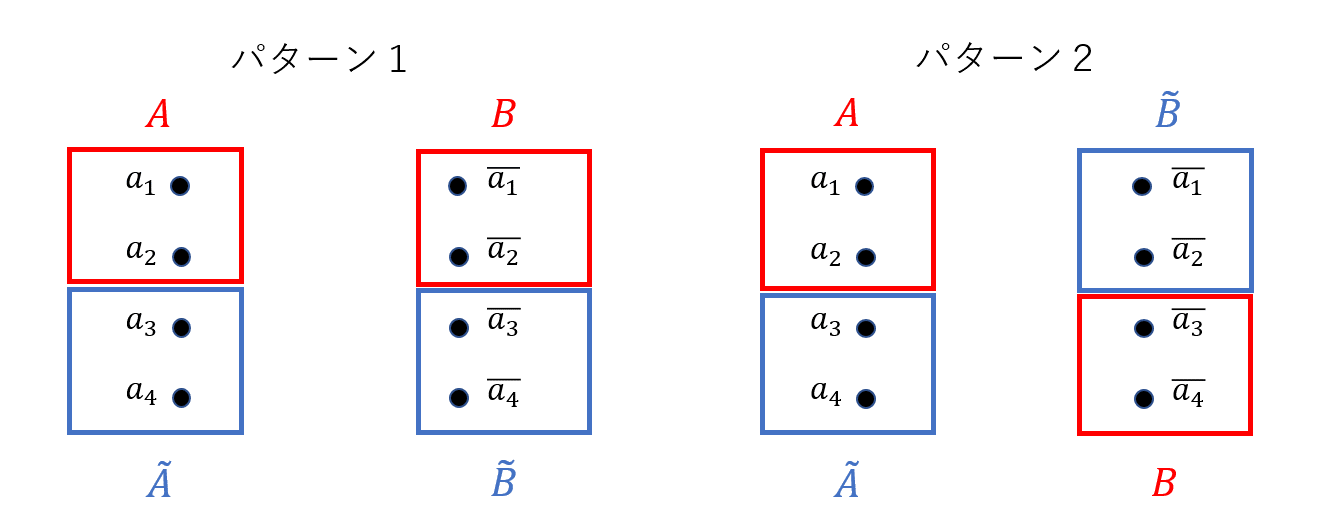
\includegraphics[width=\linewidth]{画像/k=2におけるパターン.png}
\caption{\scriptsize k=2における二分グラフの違い}
\label{k=2におけるパターン}
\end{figure}

$k=2$であるとき,$0 \le \sharp A \le 2$となる.
$\sharp A = \sharp B$である場合から考えると,$\sharp A=2$かつ$\sharp B=2$であれば,$G$に含まれる辺は,図\ref{k=2におけるパターン}パターン1のように,$\sharp\tilde{A} \times \sharp\tilde{B}=2 \times 2=4$本となる.
図\ref{k=2におけるパターン}パターン2のように,$G$に含まれる辺の2本が系のようなパターンとなる.
よって,$G$に含まれる辺の$4-2=2$本は,補題\ref{追加補題1}のようなパターンとなる.
したがって,ある$i$に対して,$p \{ x:=xy \} \preceq q_{i}$となる.
これは,仮定に矛盾する.

$\sharp A=1$かつ$\sharp B=1$であれば,$G$に含まれる辺は,$\sharp\tilde{A} \times \sharp\tilde{B}=3 \times 3=9$本となる.
$\sharp A_{1}=1,\sharp B_{1}=1$である$\tilde{G}_{1}$に含まれる辺は最大1本となる.
よって,$\tilde{G}_{2}$には$9-1=8$本の辺が含まれる.
補題\ref{追加補題1}の証明と同様に考えると,$p \{ x:= xy \} \preceq q_{2}$となる.
これは,仮定に矛盾する.

$\sharp A=0$かつ$\sharp B=0$であれば,$G$に含まれる辺は,$\sharp\tilde{A} \times \sharp\tilde{B}=4 \times 4=16$本となる.
$16 \ge 4 \times 2 + 1$より,$\tilde{G}_{1},\tilde{G}_{2}$のいずれかには,5本以上の辺が含まれる.
よって,ある$i$に対して,$p \{ x:=xy \} \preceq q_{i}$となる.
これは,仮定に矛盾する.

\begin{figure}[H]
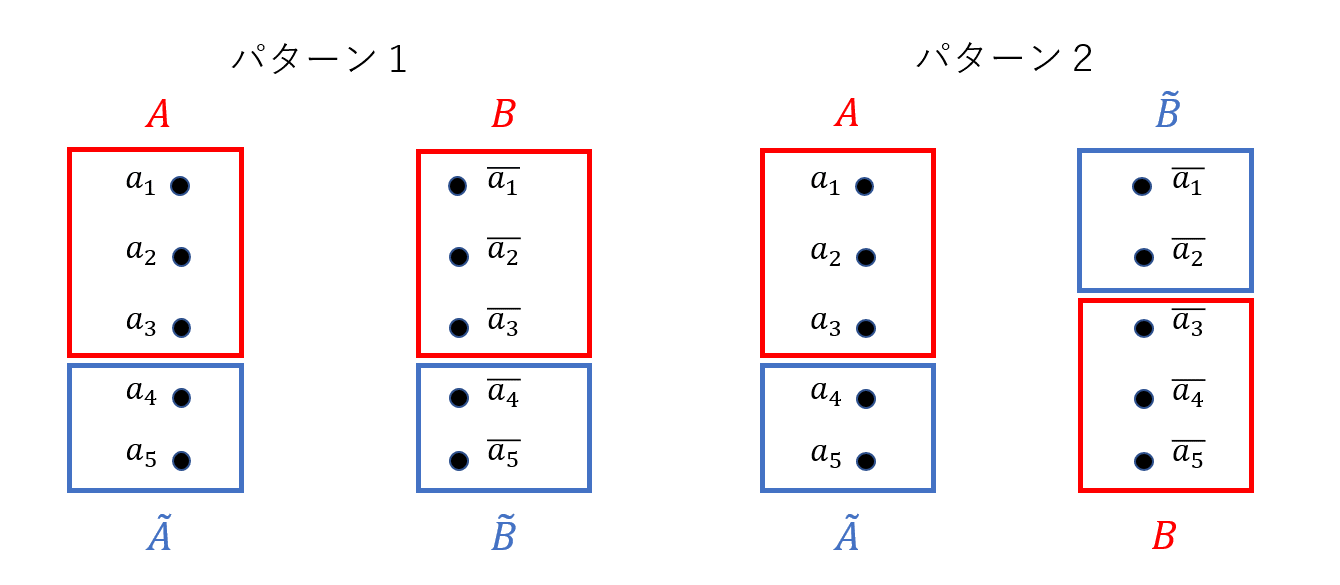
\includegraphics[width=\linewidth]{画像/k=3におけるパターン.png}
\caption{\scriptsize k=3における二分グラフの違い}
\label{k=3におけるパターン}
\end{figure}

$k=3$であるとき,$0 \le \sharp A \le 3$となる.
$\sharp A = \sharp B$である場合から考えると,$\sharp A=3$かつ$\sharp B=3$であれば,$G$に含まれる辺は,図\ref{k=3におけるパターン}パターン1のように,$\sharp\tilde{A} \times \sharp\tilde{B}=2 \times 2=4$本となる.
図\ref{k=3におけるパターン}パターン2のように,$G$に含まれる辺の3本が系のようなパターンとなる.
よって,$G$に含まれる辺の$4-3=1$本は,補題\ref{追加補題1}のようなパターンとなる.
したがって,ある$i$に対して,$p \{ x:=xy \} \preceq q_{i}$となる.
これは,仮定に矛盾する.

$\sharp A=2$かつ$\sharp B=2$であれば,$G$に含まれる辺は,$\sharp\tilde{A} \times \sharp\tilde{B}=3 \times 3=9$本となる.
$\sharp A_{i}=1,\sharp B_{i}=1$である$\tilde{G}_{i} (i=1,2)$に含まれる辺は最大2本となる.
よって,$\tilde{G}_{3}$には$9-2=7$本の辺が含まれる.
補題\ref{追加補題1}の証明と同様に考えると,$p \{ x:= xy \} \preceq q_{3}$となる.
これは,仮定に矛盾する.

$\sharp A=1$かつ$\sharp B=1$であれば,$G$に含まれる辺は,$\sharp\tilde{A} \times \sharp\tilde{B}=4 \times 4=16$本となる.
図のように,$G$に含まれる辺の1本が系のようなパターンとなる.
$16-1=15 \ge 4 \times 2 + 1$より,$\tilde{G}_{2},\tilde{G}_{3}$のいずれかには,5本以上の辺が含まれる.
よって,ある$i$に対して,$p \{ x:=xy \} \preceq q_{i}$となる.
これは,仮定に矛盾する.

$\sharp A=0$かつ$\sharp B=0$であれば,$G$に含まれる辺は,$\sharp\tilde{A} \times \sharp\tilde{B}=5 \times 5=25$本となる.
$25 \ge 4 \times 3 + 1$より,$\tilde{G}_{1},\tilde{G}_{2},\tilde{G}_{3}$のいずれかには,5本以上の辺が含まれる.
よって,ある$i$に対して,$p \{ x:=xy \} \preceq q_{i}$となる.
これは,仮定に矛盾する.

$k=2,3$のとき,$\sharp A \not = \sharp B$であれば,$\sharp A_{i}=1,\sharp B_{i}=0$または,$\sharp A_{i} =0,\sharp B_{i}=1$となる$i$が存在する.

$\sharp A_{i}=1,\sharp B_{i}=0$の場合は,図\ref{abが異なる場合}のように,$\sharp A_{i} =1,\sharp B_{i}=1$の場合と比べて,$G$に含まれる辺数は$\sharp\tilde{A}$本多くなる.

補題\ref{追加補題1}の証明と同様に考えると,$\sharp A_{i}=1,\sharp B_{i}=0$であれば,$\tilde{G}_{i}$に含まれる辺数が2以下となる.
よって,$\sharp\tilde{A} \ge 2$より,$G$に含まれる辺数が減ることはない.
$\sharp A_{i}=0,\sharp B_{i}=1$の場合も同様に考えられるため,$\sharp A \not = \sharp B$においても,仮定に矛盾する.
\end{proof}

補題\ref{追加補題1},補題\ref{補題15}より,次の定理が成り立つ.

\begin{thm}\label{定理17}
$k \ge 3$,$\sharp \Sigma \ge 2k-1$,$P \in \RPatplus,Q \in \RPat^{k}$とする.
このとき,以下の{\rm (i),(ii),(iii)}は同値である.
\[
\begin{tabular}{ll}
$(\mathrm{i})$ $S_{2}(P) \subseteq L(Q),$
$(\mathrm{ii})$ $P \sqsubseteq Q,$
$(\mathrm{iii})$ $L(P) \subseteq L(Q).$
\end{tabular}
\]
\end{thm}

\begin{proof}
(ii) $\Rightarrow$ (iii)と(iii) $\Rightarrow$ (i)は自明である.
定理\ref{定理10}より,$\sharp\Sigma \ge 2k+1$のとき,(i) $\Rightarrow$ (ii)は成り立つ.
よって,$\sharp Q=k$のとき,$\sharp\Sigma = 2k-1$または$\sharp\Sigma = 2k$の場合,(i) $\Rightarrow$ (ii)が成り立つことを,$p$に含まれる変数記号の数$n$に関する数学的帰納法により証明する.

$n=0$のとき,$S_{2}(p)= \{ p \}$であり,$p \in L(Q)$となる.よって,ある$q \in Q$に対して,$p \preceq q$となる.

$n \ge 0$個の変数記号を含む任意の正規パターンに対して題意が成り立つと仮定する.
$p$を$S_{2}(p) \subseteq L(Q)$を満たす$n+1$個の変数記号を含む正規パターンとする.
$p \not \preceq q_{i}$ ($i=1, \ldots, k$)と仮定する.
$p=p_{1}xp_{2}$ ($p_{1},p_{2}$は正規パターン,$x$は変数記号),$Q=\{ q_{1}, \ldots , q_{k} \}$を考える.
$a, b \in \Sigma$に対して,$p_{a}=p \{ x := a \}$と$p_{ab}=p \{ x := ab \}$とおく.
このとき,$p_{a},p_{ab}$は$n$個の変数記号が含まれ,$S_{2}(p_{a}) \subseteq L(Q)$かつ$S_{2}(p_{ab}) \subseteq L(Q)$が成り立つことに注意する.
帰納法の仮定より,任意の$a,b \in \Sigma$に対して,$p_{a} \preceq q_{i}$かつ$p_{ab} \preceq q_{i^{\prime}}$を満たすような$i, i^{\prime} \le k$が存在する. 
$D_{i}=\{ a \in \Sigma \mid p \{ x:=a \} \preceq q_{i} \}$ \ ($i=1, \ldots, k$)とする.
ある$i$に対して,$\sharp D_{i} \ge 3$であるとき,補題\ref{補題10}より,$p \preceq q_{i}$となる.これは仮定に矛盾する.
よって,$\sharp D_{i} \le 2$ ($i=1, \ldots, k$)となる場合を考える.
$\sharp\Sigma = 2k-1$のとき,任意の$i$に対して,$\sharp D_{i}=2$または$\sharp D_{i}=1$,$\sharp\Sigma = 2k$のとき,任意の$i$に対して,$\sharp D_{i}=2$となる.
$k \ge 3$であるとき,$2k+1 \ge k+2$となる.
よって,補題\ref{追加補題1}より,$p \{ x:=xy \} \preceq q_{i}$となる$i$が存在する.
したがって,補題\ref{補題15}より,$p \preceq q_{i}$となる.
これは仮定に矛盾する.
  
以上より,(i) $\Rightarrow$ (ii)が成り立つ.
\end{proof}

この定理\ref{定理17}より,次の系が得られる.

\begin{col}\label{命題18}
$k \ge 3$,$\sharp\Sigma \ge 2k-1$,$P \in \mathcal{RP}^{+}$とする.このとき,$S_{2}(P)$は$\mathcal{RPL}^{k}$における$L(P)$の特徴集合である.
\end{col}

\begin{lem}[Sato et al.\cite{Sato1}]\label{補題19}
$\sharp\Sigma \le 2k-2$とする.このとき,$\mathcal{RP}^{k}$は包含に関するコンパクト性を持たない.
\end{lem}

\begin{proof}
$\Sigma = \{ a_{1}, \ldots , a_{k-1}, b_{1}, \ldots , b_{k-1} \}$を$(2k-2)$個の定数記号から成る集合,$p, q_{i}$を正規パターン,$w_{i}~(i = 1, \ldots , k-1)$を例\ref{例題1}と同様に定義された記号列とする.
$q_{k} = x_{1}a_{1}w_{1}xyw_{1}b_{1}x_{2}$とする.
例\ref{例題1}で示した通り,$p \{ x := a_{i} \} \preceq q_{i}$かつ$p \{ x := b_{i} \} \preceq q_{i}~(i=1,2, \ldots ,k-1)$であるとき,$S_{1}(p) \subseteq \bigcup^{k-1}_{i=1} L(q_{i})$となる. 
一方で,任意の$w$ $(|w| \ge 2)$に対して,$p \{ x:= w \} \preceq q_{k}$となる. 
すなわち,$L(p) \subseteq L(Q)$である.
しかし,$p \not \preceq q_{i}$であるため,$L(p) \not \subseteq L(q_{i}) (i=1,2, \ldots k)$である.
したがって,$\RPatkei$は包含に関するコンパクト性を持たない.
\end{proof}

定理\ref{定理17}と補題\ref{補題19}より,次の定理が成り立つ.

\begin{thm}
$k \ge 3$とし,$\sharp\Sigma \ge 2k-1$とする.
このとき,$\RPat^{k}$は包含に関してコンパクト性を持つ.
\end{thm}

$k=2$のとき,次の定理が成り立つ.

\begin{thm}\label{補題21}
$\sharp \Sigma \ge 4$とし,$P \in \RPatplus$,$Q \in \RPat^{2}$とする.
このとき,以下の{\rm (i),(ii),(iii)}は同値である.
\[
\begin{tabular}{ll}
$(\mathrm{i})$ $S_{2}(P) \subseteq L(Q),$
$(\mathrm{ii})$ $P \sqsubseteq Q,$
$(\mathrm{iii})$ $L(P) \subseteq L(Q).$
\end{tabular}
\]
\end{thm}

\begin{proof}
(ii) $\Rightarrow$ (iii)と(iii) $\Rightarrow$ (i)は自明に成り立つ.
よって,(i) $\Rightarrow$ (ii)が成り立つことを示す.
$Q= \{ q_{1}, q_{2} \}$とするとき,$p$に含まれる変数記号の数$n$に関する数学的帰納法で示す.\\
\noindent (1) $n=0$のとき,$p$は定数記号列となるので$S_{2}(p)= \{ p \}$となり
(i)より,$p \in L(Q)$となる.
よって,ある$q \in Q$に対して$p \preceq q$となる.\\
\noindent (2) $n=k$個の変数記号を含むすべての正規パターンに対して有効であると仮定する.
そして,$p$を$S_{2}(p) \subseteq L(Q)$を満たす$(n+1)$個の変数記号を含む正規パターンとする.

$p \not \preceq q_{i}$ ($i=1, 2$)と仮定する.
$p=p_{1}xp_{2}$ ($p_{1}, p_{2}$は正規パターン,$x$は変数記号)を考える.
$a, b \in \Sigma$に対して,$p_{a}=p \{ x := a \}$,$p_{ab}=p \{ x := ab \}$とおく.
このとき,$p_{a},p_{ab}$は$n$個の変数記号が含まれ,$S_{2}(p_{a}) \subseteq L(Q)$,$S_{2}(p_{ab}) \subseteq L(Q)$が成り立つことに注意する.
帰納法の仮定より,任意の$a, b \in \Sigma$に対して,$p_{a} \preceq q_{i}, p_{ab} \preceq q_{i^{\prime}}$を満たすような$i, i^{\prime} \le k$が存在する.

ある$i$に対して$\sharp D_{i} \ge 3$のとき,補題\ref{補題10}より,$p \preceq q_{i}$となる.
よって,任意の$i$に対して,$\sharp D_{i} \le 2$となる.
したがって,$\sharp D_{1}=2$かつ$\sharp D_{2}=2$となる場合を考える.

$\sharp \Sigma = k+2$であるとき,$k=2$より,$\sharp \Sigma =4$となる.
よって,補題\ref{追加補題1}より,ある$i$に対して,$p \{ x:=xy \} \preceq q_{i}$となる.
したがって,補題\ref{補題15}より,$p \preceq q_{i}$となる.
これは,仮定に矛盾する.

以上より,(i) $\Rightarrow$ (ii)が成り立つ.
\end{proof}

次の例は,$k = 2$における定理\ref{補題21}の反例である.
\begin{ex}\label{反例thm17}
$\Sigma= \{a, b, c \}$を$3$つの定数記号から成る集合,$p,q_{1},q_{2}$を正規パターン,$x,x^{\prime},x^{\prime\prime}$を変数記号とする.
\begin{eqnarray*}
p = x^{\prime}axbx^{\prime\prime},
q_{1} = x^{\prime}abx^{\prime\prime},
q_{2} = x^{\prime}cx^{\prime\prime}.
\end{eqnarray*}
$w \in \Sigma^{+}$とする.$w$に$c$が含まれるとき,$p \{ x:=w \} \preceq q_{2}$となり,$c$が含まれないとき,$p \{ x:=w \} \preceq q_{1}$となる.
よって,$L(p) \subseteq L(q_{1}) \cup L(q_{2})$である.
しかし,$p \not \preceq q_{1}$かつ$p \not \preceq q_{2}$である.
\end{ex}

定理\ref{補題21}より,次の2つの系が成り立つ.
\begin{col}
$\sharp\Sigma \ge 4$とし,$P \in \RPatplus$とする.
このとき,$S_{2}(P)$は,$\RPatL^{2}$における$L(P)$の特徴集合である.
\end{col}

\begin{col}
$\sharp\Sigma \ge 4$とする.このとき,クラス$\mathcal{RP}^{2}$は包含に関してコンパクト性を持つ.
\end{col}

